\documentclass[%
 reprint, amsmath,amssymb, aps, prb, ]{revtex4-2}
\usepackage{graphicx}
\usepackage{bm}
\usepackage{physics}
\usepackage[colorlinks=true,
            linkcolor=blue, filecolor=blue, urlcolor=blue, citecolor=blue]{hyperref}
\usepackage{caption}
\captionsetup[figure]{justification=raggedright, labelfont={bf}, name={Fig.}, labelsep=period}
\captionsetup[table]{labelfont={bf}, name={Table}, labelsep=period}
\numberwithin{equation}{section}
\tolerance=1000
\emergencystretch=1em
\hyphenpenalty=3000
\exhyphenpenalty=3000
\flushbottom
\usepackage[final]{microtype}
\usepackage{ragged2e}
\usepackage{booktabs}
\usepackage{enumitem}
\usepackage{amsthm}
\newtheorem{theorem}{Theorem}[section]
\usepackage{xcolor}
\usepackage{tikz}
\usetikzlibrary{arrows.meta, calc, 3d, shadings, positioning,
                decorations.pathmorphing, decorations.markings,
                shapes.geometric}
% --- Custom Macros ---
\newcommand{\iphase}{\theta}
\newcommand{\omZB}{\omega_{\text{ZB}}}
\newcommand{\EphS}{E_{\text{ph}}}
\newcommand{\Ezp}{E_0/2}
\newcommand{\Egrad}{\Delta E_{\text{AB}}}
\newcommand{\FF}{\mathbf{F}}
\newcommand{\WL}{\mathcal{W}}
\newcommand{\hodge}{\star}
\newcommand{\lambdaC}{\lambda_{\mathrm{C}}}

% ========================================
% TikZ macro: harmonic oscillator reinterpretation (side-by-side)
% Left: conventional QM / Right: 0-Sphere interpretation
% ========================================
\newcommand{\figHOreinterpret}{%
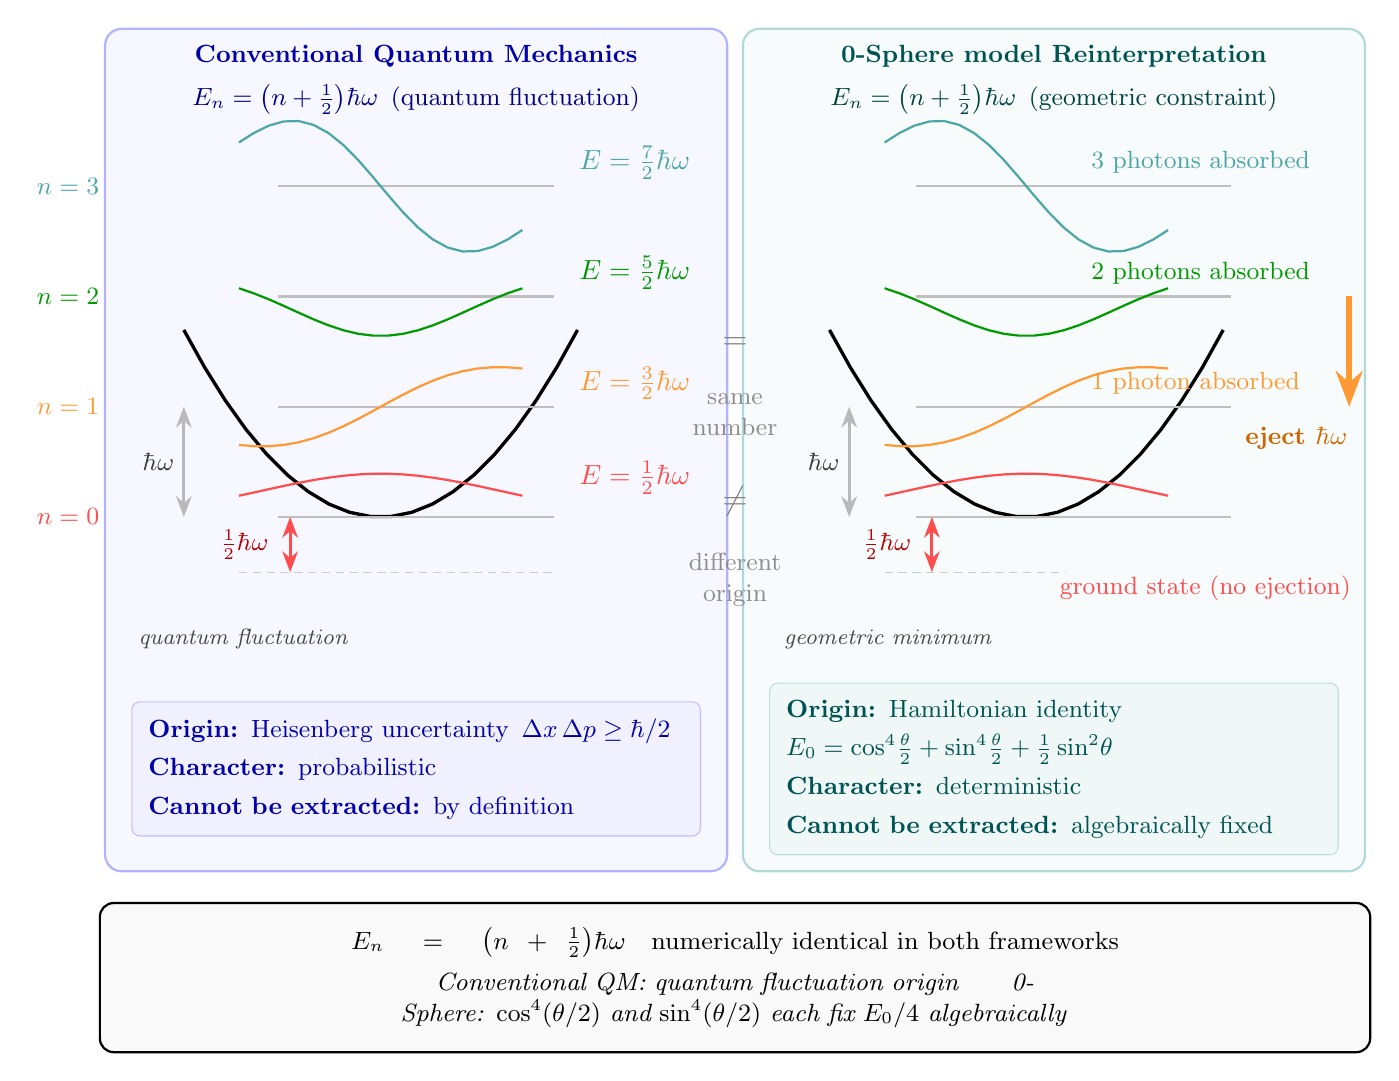
\begin{tikzpicture}[>=Stealth, font=\small]

% Vertical layout (n=0..3 only):
%   Potential minimum:  y = -0.70  (parabola 0.38x^2 - 0.70)
%   n=0..3 at y = 0.00 / 1.40 / 2.80 / 4.20   (spacing = 1.40 = hbar*omega)
%   ZPE gap: -0.70 -> 0.00 = 0.70 = (1/2)hbar*omega   [ratio 1:2, exact]
%
% Wavefunctions: Hermite H_n basis, a=0.22, domain [-2.5, 2.5]
%   n=0:  A * exp(-a x^2)                      Gaussian, 0 nodes
%   n=1:  A * x * exp(-a x^2)                  H_1,      1 node  at x=0
%   n=2:  A * (2a x^2 - 1) * exp(-a x^2)       H_2,      2 nodes
%   n=3:  A * x*(2a x^2 - 3) * exp(-a x^2)     H_3,      3 nodes
% Amplitudes: 0.55 / 0.55 / 0.50 / 0.40

%%====================================================
%% LEFT BOX  (Conventional QM)
%%====================================================
\draw[thick, rounded corners=6pt, fill=blue!3, draw=blue!30]
  (-8.0, -4.5) rectangle (-0.1, 6.2);
\node[font=\small\bfseries, blue!65!black] at (-4.05, 5.85)
  {Conventional Quantum Mechanics};
\node[font=\small, blue!50!black] at (-4.05, 5.30)
  {$E_n = \bigl(n+\tfrac{1}{2}\bigr)\hbar\omega$\enspace(quantum fluctuation)};

%% Potential well
\draw[black, very thick, domain=-2.5:2.5, samples=20]
  plot ({-4.5+\x}, {0.38*\x*\x + 0.00});

%% Dashed line: potential minimum
\draw[gray!40, densely dashed, thin] (-6.3, -0.70) -- (-2.3, -0.70);

%% n=0
\draw[gray!50, thick] (-5.8, 0.00) -- (-2.3, 0.00);
\node[anchor=east, font=\small, red!70] at (-7.95, 0.00) {$n=0$};
\node[anchor=west, font=\normalsize, red!70] at (-2.1, 0.50)
  {$E = \tfrac{1}{2}\hbar\omega$};
\draw[red!70, thick, domain=-1.8:1.8, samples=20]
  plot ({-4.5+\x}, {0.00 + 0.55*exp(-0.22*\x*\x)});

%% n=1
\draw[gray!50, thick] (-5.8, 1.40) -- (-2.3, 1.40);
\node[anchor=east, font=\small, orange!80] at (-7.95, 1.40) {$n=1$};
\node[anchor=west, font=\normalsize, orange!80] at (-2.1, 1.70)
  {$E = \tfrac{3}{2}\hbar\omega$};
\draw[orange!80, thick, domain=-1.8:1.8, samples=20]
  plot ({-4.5+\x}, {1.40 + 0.55*\x*exp(-0.22*\x*\x)});

%% n=2
\draw[gray!50, thick] (-5.8, 2.80) -- (-2.3, 2.80);
\node[anchor=east, font=\small, green!60!black] at (-7.95, 2.80) {$n=2$};
\node[anchor=west, font=\normalsize, green!60!black] at (-2.1, 3.10)
  {$E = \tfrac{5}{2}\hbar\omega$};
\draw[green!60!black, thick, domain=-1.8:1.8, samples=20]
  plot ({-4.5+\x}, {2.80 + 0.50*(2*0.22*\x*\x - 1)*exp(-0.22*\x*\x)});

%% n=3
\draw[gray!50, thick] (-5.8, 4.20) -- (-2.3, 4.20);
\node[anchor=east, font=\small, teal!70] at (-7.95, 4.20) {$n=3$};
\node[anchor=west, font=\normalsize, teal!70] at (-2.1, 4.50)
  {$E = \tfrac{7}{2}\hbar\omega$};
\draw[teal!70, thick, domain=-1.8:1.8, samples=20]
  plot ({-4.5+\x}, {4.20 + 0.40*\x*(2*0.22*\x*\x - 3)*exp(-0.22*\x*\x)});

%% Annotations (left outer margin)
\draw[red!70, <->, line width=1.0pt] (-5.65, -0.70) -- (-5.65, 0.00);
\node[anchor=east, font=\small, red!70!black] at (-5.80, -0.35)
  {$\tfrac{1}{2}\hbar\omega$};
\draw[gray!55, <->, line width=1.0pt] (-7.00, 0.00) -- (-7.00, 1.40);
\node[anchor=east, font=\small, gray!45!black] at (-7.00, 0.70)
  {$\hbar\omega$};
\node[anchor=west, font=\footnotesize, gray!55!black] at (-7.70, -1.55)
  {\textit{quantum fluctuation}};

%% Key result box
\node[draw=blue!25, rounded corners=3pt, fill=blue!6,
  font=\small, text=blue!65!black, inner sep=6pt, text width=6.8cm,
  align=left] at (-4.05, -3.20) {%
  \textbf{Origin:} Heisenberg uncertainty\enspace$\Delta x\,\Delta p \geq \hbar/2$\\[3pt]
  \textbf{Character:} probabilistic\\[3pt]
  \textbf{Cannot be extracted:} by definition};

%%====================================================
%% RIGHT BOX  (0-Sphere)
%%====================================================
\draw[thick, rounded corners=6pt, fill=teal!3, draw=teal!30]
  (0.1, -4.5) rectangle (8.0, 6.2);
\node[font=\small\bfseries, teal!65!black] at (4.05, 5.85)
  {0-Sphere model Reinterpretation};
\node[font=\small, teal!50!black] at (4.05, 5.30)
  {$E_n = \bigl(n+\tfrac{1}{2}\bigr)\hbar\omega$\enspace(geometric constraint)};

%% Potential well
\draw[black, very thick, domain=-2.5:2.5, samples=20]
  plot ({3.7+\x}, {0.38*\x*\x + 0.00});

%% Dashed line: potential minimum
\draw[gray!40, densely dashed, thin] (1.9, -0.70) -- (4.2, -0.70);

%% n=0
\draw[gray!50, thick] (2.3, 0.00) -- (6.3, 0.00);
\node[anchor=west, font=\small, red!70] at (4.0, -0.90)
  {ground state (no ejection)};
\draw[red!70, thick, domain=-1.8:1.8, samples=20]
  plot ({3.7+\x}, {0.00 + 0.55*exp(-0.22*\x*\x)});

%% n=1
\draw[gray!50, thick] (2.3, 1.40) -- (6.3, 1.40);
\node[anchor=west, font=\small, orange!80] at (4.4, 1.70)
  {1 photon absorbed};
\draw[orange!80, thick, domain=-1.8:1.8, samples=20]
  plot ({3.7+\x}, {1.40 + 0.55*\x*exp(-0.22*\x*\x)});

%% n=2
\draw[gray!50, thick] (2.3, 2.80) -- (6.3, 2.80);
\node[anchor=west, font=\small, green!60!black] at (4.4, 3.10)
  {2 photons absorbed};
\draw[green!60!black, thick, domain=-1.8:1.8, samples=20]
  plot ({3.7+\x}, {2.80 + 0.50*(2*0.22*\x*\x - 1)*exp(-0.22*\x*\x)});

%% n=3  (REVISED: removed tentative Y_2^0 label; mode identification is open)
\draw[gray!50, thick] (2.3, 4.20) -- (6.3, 4.20);
\node[anchor=west, font=\small, teal!70] at (4.4, 4.50)
  {3 photons absorbed};
\draw[teal!70, thick, domain=-1.8:1.8, samples=20]
  plot ({3.7+\x}, {4.20 + 0.40*\x*(2*0.22*\x*\x - 3)*exp(-0.22*\x*\x)});

%% Annotations (right inner margin)
\draw[red!70, <->, line width=1.0pt] (2.50, -0.70) -- (2.50, 0.00);
\node[anchor=west, font=\small, red!70!black] at (1.50, -0.35)
  {$\tfrac{1}{2}\hbar\omega$};
\draw[gray!55, <->, line width=1.0pt] (1.45, 0.00) -- (1.45, 1.40);
\node[anchor=west, font=\small, gray!45!black] at (0.80, 0.70)
  {$\hbar\omega$};
\node[anchor=west, font=\footnotesize, gray!55!black] at (0.50, -1.55)
  {\textit{geometric minimum}};

%% Ejection arrow n=2 -> n=1
\draw[->, orange!80, line width=2.2pt] (7.8, 2.80) -- (7.8, 1.40);
\node[anchor=east, font=\small\bfseries, orange!80!black]
  at (7.90, 1.00) {eject $\hbar\omega$};

%% Key result box
\node[draw=teal!25, rounded corners=3pt, fill=teal!6,
  font=\small, text=teal!65!black, inner sep=6pt, text width=6.8cm,
  align=left] at (4.05, -3.20) {%
  \textbf{Origin:} Hamiltonian identity\\[3pt]
  $E_0 = \cos^4\!\tfrac{\iphase}{2} + \sin^4\!\tfrac{\iphase}{2} + \tfrac{1}{2}\sin^2\!\iphase$\\[3pt]
  \textbf{Character:} deterministic\\[3pt]
  \textbf{Cannot be extracted:} algebraically fixed};

%%====================================================
%% CENTRE — between boxes
%%====================================================
\node[font=\large\bfseries, black!50] at (0, 2.2) {$=$};
\node[font=\small, black!45, align=center] at (0, 1.3) {same\\number};
\node[font=\large\bfseries, black!50] at (0, 0.2) {$\neq$};
\node[font=\small, black!45, align=center] at (0, -0.8) {different\\origin};

%%====================================================
%% BOTTOM STRIP
%%====================================================
\node[draw, thick, rounded corners=5pt, fill=gray!5,
  text width=15.5cm, font=\small, align=center, inner sep=9pt]
  at (0, -5.85) {
  $E_n = \bigl(n + \tfrac{1}{2}\bigr)\hbar\omega$\quad numerically identical in both frameworks\\[4pt]
  \textit{Conventional QM: quantum fluctuation origin}\qquad
  \textit{0-Sphere: $\cos^4(\theta/2)$ and $\sin^4(\theta/2)$ each fix $E_0/4$ algebraically}
};

\end{tikzpicture}%
}

% ========================================
% TikZ macro: photon-sphere SHM and ejection   (RESTORED)
% ========================================
\newcommand{\figEjectionMechanism}{%
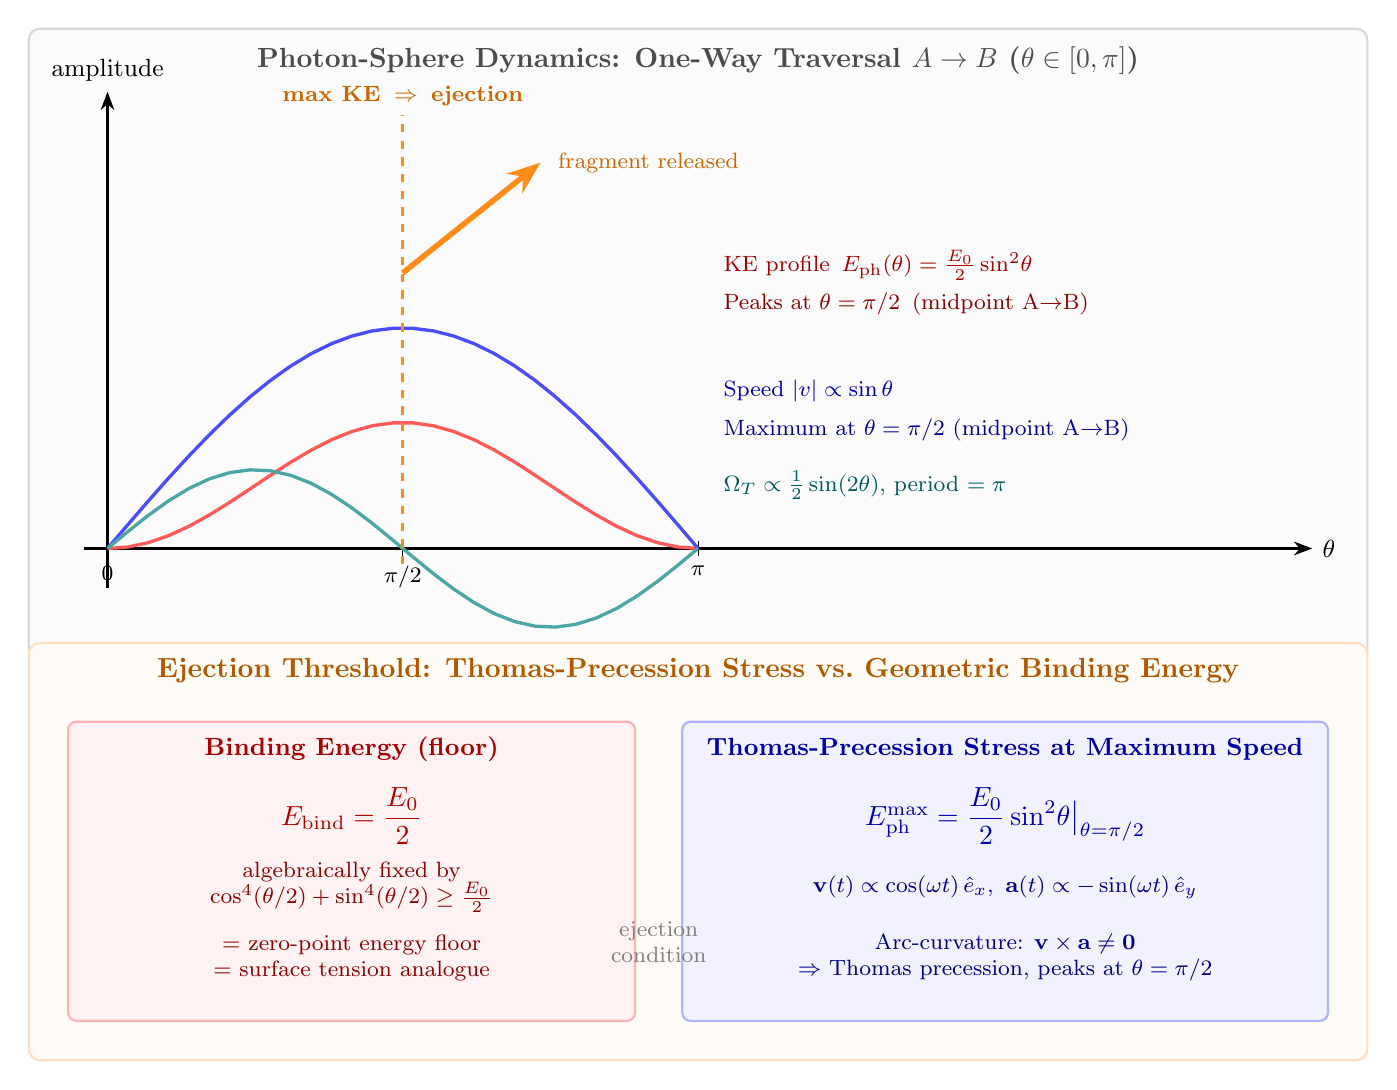
\begin{tikzpicture}[>=Stealth, font=\small]

%%====================================================
%% TOP PANEL: kinematic profiles over [0, pi]
%%====================================================
\draw[thick, rounded corners=4pt, fill=gray!3, draw=gray!30]
  (-8.5, -0.5) rectangle (8.5, 7.6);
\node[font=\normalsize\bfseries, black!70] at (0, 7.2)
  {Photon-Sphere Dynamics: One-Way Traversal $A \to B$ ($\theta \in [0,\pi]$)};

%% Axes
\draw[thick, ->] (-7.8, 1.0) -- (7.8, 1.0) node[right] {$\theta$};
\draw[thick, ->] (-7.5, 0.5) -- (-7.5, 6.8) node[above] {amplitude};

%% Tick marks on x-axis
\foreach \xv/\lab in {-7.5/{$0$}, -3.75/{$\pi/2$}, 0/{$\pi$}}{
  \draw[thin] (\xv, 0.9) -- (\xv, 1.1);
  \node[below, font=\footnotesize] at (\xv, 0.9) {\lab};
}

%% KE profile E_ph(theta) = (E0/2) sin^2(theta)
\draw[red!65, very thick, domain=-7.5:0, samples=30]
  plot (\x, {1.0 + 1.6*(1 - cos(2 * (\x + 7.5) / 7.5 * 180)) / 2});
\node[anchor=west, font=\footnotesize, red!65!black] at (0.2, 4.6)
  {KE profile\enspace$E_{\text{ph}}(\theta) = \tfrac{E_0}{2}\sin^2\!\theta$};
\node[anchor=west, font=\footnotesize, red!55!black] at (0.2, 4.1)
  {Peaks at $\theta = \pi/2$\enspace(midpoint A$\to$B)};

%% Speed v(theta) ~ sin(theta)
\draw[blue!70, very thick, domain=-7.5:0, samples=30]
  plot (\x, {1.0 + 2.8 * sin((\x + 7.5) / 7.5 * 180)});
\node[anchor=west, font=\footnotesize, blue!70!black] at (0.2, 3.0)
  {Speed $|v| \propto \sin\theta$};
\node[anchor=west, font=\footnotesize, blue!60!black] at (0.2, 2.5)
  {Maximum at $\theta = \pi/2$ (midpoint A$\to$B)};

%% Thomas angular velocity Omega_T ~ (1/2)sin(2*theta)
\draw[teal!70, very thick, domain=-7.5:0, samples=30]
  plot (\x, {1.0 + 2.0 * 0.5 * sin(2 * (\x + 7.5) / 7.5 * 180)});
\node[anchor=west, font=\footnotesize, teal!70!black] at (0.2, 1.8)
  {$\Omega_T \propto \tfrac{1}{2}\sin(2\theta)$, period $= \pi$};

%% Ejection marker at pi/2
\draw[orange!90, very thick, dashed] (-3.75, 0.8) -- (-3.75, 6.5);
\node[anchor=south, font=\footnotesize\bfseries, orange!80!black] at (-3.75, 6.5)
  {max KE\enspace$\Rightarrow$\enspace ejection};
\draw[->, orange!90, very thick, line width=2pt]
  (-3.75, 4.5) -- (-2.0, 5.9);
\node[anchor=west, font=\footnotesize, orange!80!black] at (-1.9, 5.9)
  {fragment released};

%%====================================================
%% BOTTOM PANEL: ejection threshold condition
%%====================================================
\draw[thick, rounded corners=4pt, fill=orange!3, draw=orange!25]
  (-8.5, -5.5) rectangle (8.5, -0.2);
\node[font=\normalsize\bfseries, orange!70!black] at (0, -0.55)
  {Ejection Threshold: Thomas-Precession Stress vs.\ Geometric Binding Energy};

%% Left: binding energy E_0/2
\draw[thick, rounded corners=3pt, fill=red!5, draw=red!30]
  (-8.0, -5.0) rectangle (-0.8, -1.2);
\node[font=\small\bfseries, red!65!black] at (-4.4, -1.55)
  {Binding Energy (floor)};
\node[font=\normalsize, red!70!black] at (-4.4, -2.4)
  {$E_{\text{bind}} = \dfrac{E_0}{2}$};
\node[font=\footnotesize, red!55!black, align=center] at (-4.4, -3.3)
  {algebraically fixed by\\$\cos^4(\theta/2) + \sin^4(\theta/2) \geq \tfrac{E_0}{2}$};
\node[font=\footnotesize, red!55!black, align=center] at (-4.4, -4.2)
  {= zero-point energy floor\\= surface tension analogue};

%% Right: kinetic stress at max speed
\draw[thick, rounded corners=3pt, fill=blue!5, draw=blue!30]
  (-0.2, -5.0) rectangle (8.0, -1.2);
\node[font=\small\bfseries, blue!65!black] at (3.9, -1.55)
  {Thomas-Precession Stress at Maximum Speed};
\node[font=\normalsize, blue!70!black] at (3.9, -2.4)
  {$E_{\text{ph}}^{\max} = \dfrac{E_0}{2}\sin^2\!\theta\big|_{\theta=\pi/2}$};
\node[font=\footnotesize, blue!55!black, align=center] at (3.9, -3.3)
  {$\mathbf{v}(t) \propto \cos(\omega t)\,\hat{e}_x$,\enspace$\mathbf{a}(t) \propto {-}\sin(\omega t)\,\hat{e}_y$};
\node[font=\footnotesize, blue!55!black, align=center] at (3.9, -4.2)
  {Arc-curvature: $\mathbf{v} \times \mathbf{a} \neq \mathbf{0}$\\$\Rightarrow$ Thomas precession, peaks at $\theta=\pi/2$};

%% Threshold symbol
\node[font=\large\bfseries, black!55] at (-0.5, -3.1) {$\gtrless$};
\node[font=\footnotesize, black!50, align=center] at (-0.5, -4.0)
  {ejection\\condition};

\end{tikzpicture}%
}

% ========================================
% TikZ macro: standing-wave excitation modes  (v2.1, enhanced)
% New figure added at §3.2.2 to show modal structure and
% n=0 (reference) vs n>=1 (actual ejection) distinction.
% ========================================
\newcommand{\figStandingWaves}{%
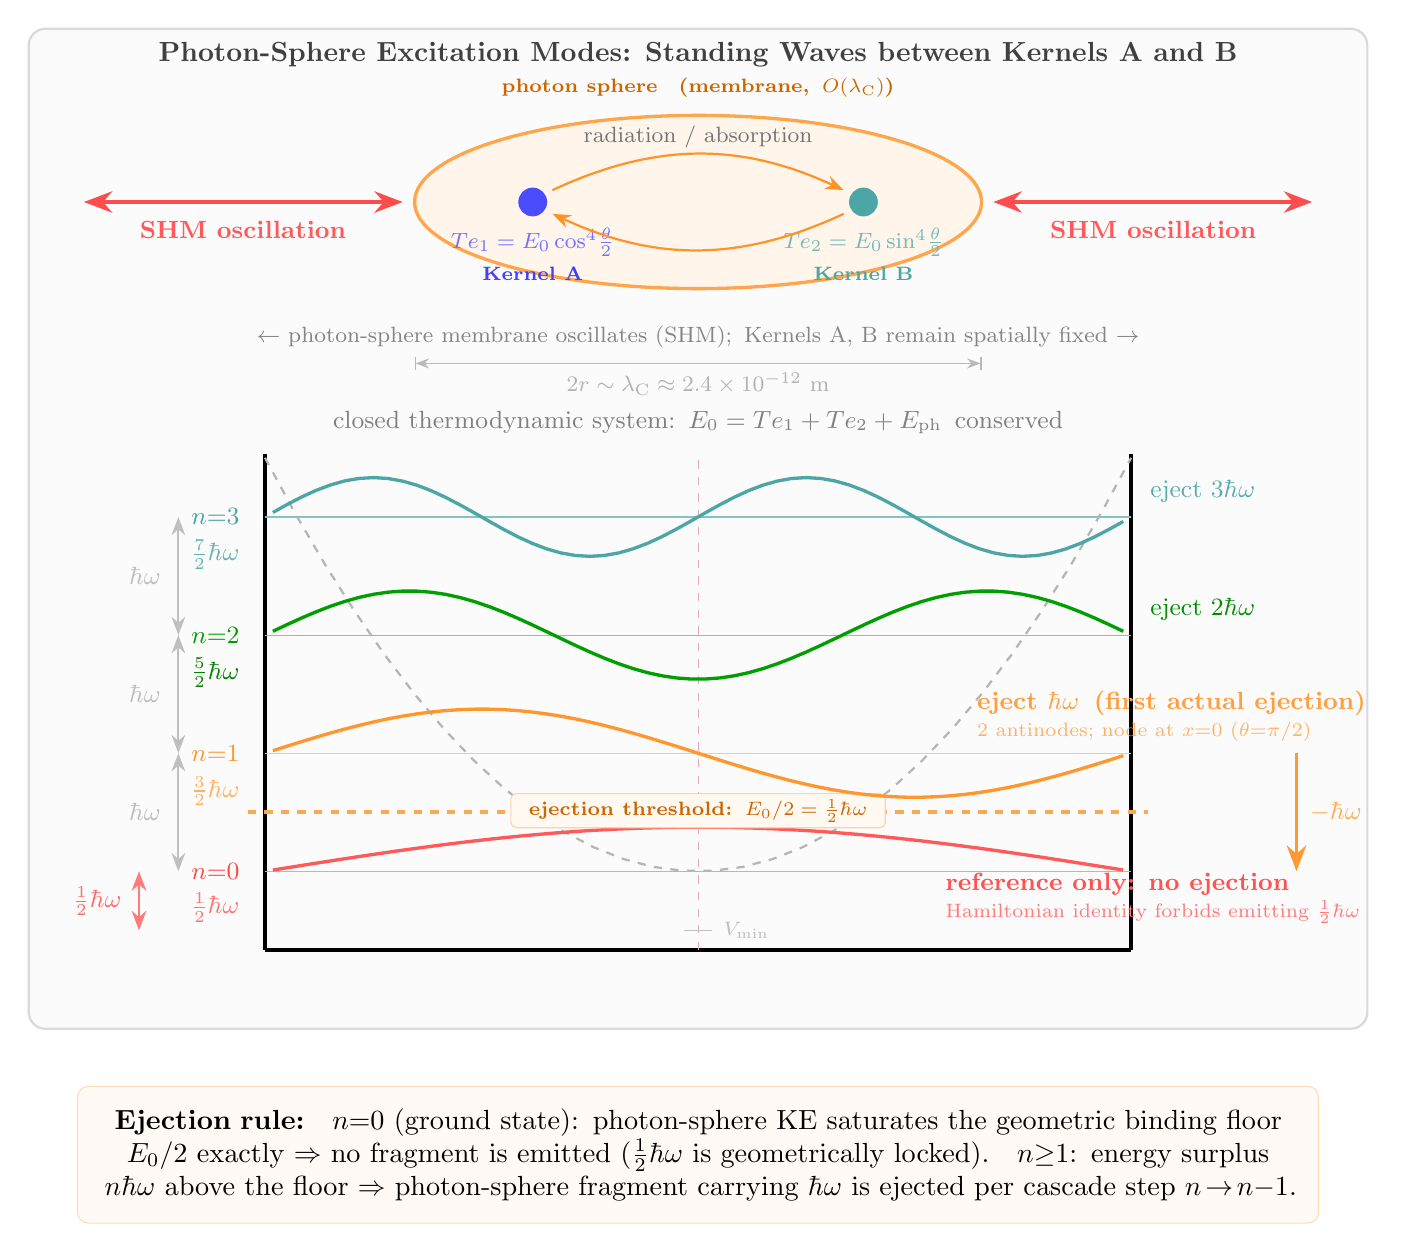
\begin{tikzpicture}[>=Stealth, font=\small]

%%====================================================
%% OUTER BOX + TITLE
%% Extended top: 8.8 -> 11.8  (3 units extra for schematic)
%%====================================================
\draw[thick, rounded corners=6pt, fill=gray!3, draw=gray!30]
  (-8.5, -0.9) rectangle (8.5, 11.8);
\node[font=\normalsize\bfseries, black!75] at (0, 11.47)
  {Photon-Sphere Excitation Modes: Standing Waves between Kernels A and B};

%%====================================================
%% SCHEMATIC: soap-bubble photon sphere containing Kernels A and B
%% Vertical centre raised to y = 9.8 (was 7.45)
%% Ellipse semi-axes: 3.6 x 1.10  (slightly taller for clearance)
%% [2026-04-01] Entire schematic shifted +0.8 (= 8 mm) upward
%%====================================================
%% --- Photon-sphere membrane (soap bubble, ellipse) ---
\draw[orange!70, very thick, fill=orange!8]
  (0, 9.60) ellipse (3.6 and 1.10);
%% --- Membrane label: above the ellipse ---
\node[font=\scriptsize\bfseries, orange!80!black, anchor=south]
  at (0, 10.80) {photon sphere \enspace (membrane,\enspace $O(\lambdaC)$)};
%% --- Kernel A (left internal point, SPATIALLY FIXED) ---
\filldraw[blue!70] (-2.10, 9.60) circle (5pt);
\node[font=\scriptsize\bfseries, blue!75, anchor=north]
  at (-2.10, 8.90) {Kernel A};
\node[font=\footnotesize, blue!55, anchor=south]
  at (-2.10, 8.78) {$Te_1 = E_0\cos^4\!\tfrac{\theta}{2}$};
%% --- Kernel B (right internal point, SPATIALLY FIXED) ---
\filldraw[teal!70] (2.10, 9.60) circle (5pt);
\node[font=\scriptsize\bfseries, teal!70, anchor=north]
  at (2.10, 8.90) {Kernel B};
\node[font=\footnotesize, teal!55, anchor=south]
  at (2.10, 8.78) {$Te_2 = E_0\sin^4\!\tfrac{\theta}{2}$};
%% --- Radiation arrows A <-> B ---
\draw[->, orange!85, thick, bend left=25]
  (-1.85, 9.75) to
  node[above, font=\footnotesize, black!55, inner sep=2pt] {radiation / absorption}
  (1.85, 9.75);
\draw[->, orange!85, thick, bend left=25]
  (1.85, 9.45) to (-1.85, 9.45);
%% --- SHM double-arrows outside membrane (photon sphere oscillates; kernels do NOT) ---
\draw[<->, red!70, very thick, line width=1.6pt]
  (-7.80, 9.60) -- (-3.75, 9.60);
\draw[<->, red!70, very thick, line width=1.6pt]
  (3.75, 9.60) -- (7.80, 9.60);
\node[font=\small\bfseries, red!65, anchor=north] at (-5.78, 9.48)
  {SHM oscillation};
\node[font=\small\bfseries, red!65, anchor=north] at (5.78, 9.48)
  {SHM oscillation};
%% Note: photon sphere membrane oscillates; kernels A, B remain spatially fixed
\node[font=\footnotesize, black!48, align=center] at (0, 7.88)
  {$\leftarrow$ photon-sphere membrane oscillates (SHM);\enspace
   Kernels A, B remain spatially fixed $\rightarrow$};
%% --- Scale annotation: below the ellipse ---
\draw[gray!55, thin, |<->|]
  (-3.60, 7.55) -- (3.60, 7.55)
  node[midway, below, font=\footnotesize, gray!60]
  {$2r \sim \lambdaC \approx 2.4\times10^{-12}\ \text{m}$};
%% --- Closed-system annotation ---
\node[font=\small, black!50, align=center] at (0, 6.80)
  {closed thermodynamic system:\enspace
   $E_0 = Te_1 + Te_2 + E_{\text{ph}}$\enspace conserved};

%%====================================================
%% POTENTIAL WELL
%%  Layout (hbar*omega = 1.50 in y-units):
%%    V_min at y = 0.35
%%    ZPE = (1/2)*1.50 = 0.75  =>  n=0 level at y = 1.10
%%    n=1 at y = 2.60,  n=2 at y = 4.10,  n=3 at y = 5.60
%%    Parabola: V(x) = 0.1736 x^2 + 0.35  [V(5.5)=5.60]
%%
%%  Standing waves (particle-in-box on [-5.5, 5.5]):
%%    psi_n(x) = A_n * sin((n+1)*180*(x+5.5)/11)  [TikZ degrees]
%%    n=0: 0 internal nodes  (single arch)
%%    n=1: 1 internal node   (full sine)
%%    n=2: 2 internal nodes  (3/2 arches)
%%    n=3: 3 internal nodes  (2 full cycles)
%%====================================================

%% Walls + floor
\draw[very thick] (-5.5, 0.10) -- (-5.5, 6.40);
\draw[very thick] ( 5.5, 0.10) -- ( 5.5, 6.40);
\draw[very thick] (-5.5, 0.10) -- ( 5.5, 0.10);

%% Midpoint vertical line: x=0 corresponds to theta=pi/2 (max speed, peak ejection stress)
\draw[purple!35, dashed, thin] (0, 0.10) -- (0, 6.40);

%% Harmonic potential (dashed parabola) — reference curve only; 
%% classical turning points widen with n (no wall constraint)
\draw[gray!58, thick, dashed, domain=-5.50:5.50, samples=30]
  plot (\x, {0.1736*\x*\x + 1.10});

%% V_min marker
\draw[gray!48, thin] (-0.18, 0.35) -- (0.18, 0.35);
\node[anchor=west, font=\scriptsize, gray!52] at (0.20, 0.35) {$V_{\min}$};

%%
%% --- n = 0  (ground state: floor saturated, no ejection) ---
%%
\draw[red!40, thin] (-5.5, 1.10) -- (5.5, 1.10);
\node[anchor=east, font=\small\bfseries, red!72] at (-5.70, 1.10) {$n{=}0$};
\node[anchor=east, font=\small,         red!55] at (-5.70, 0.64)
  {$\tfrac{1}{2}\hbar\omega$};
%% Waveform: single arch, 0 internal nodes
\draw[red!65, very thick, domain=-5.4:5.4, samples=60]
  plot (\x, {1.10 + 0.56*sin(180*(\x+5.5)/11)});
\node[anchor=west, font=\small\bfseries, red!68] at (3.02, 0.94)
  {reference only: no ejection};
\node[anchor=west, font=\scriptsize,     red!52] at (3.02, 0.58)
  {Hamiltonian identity forbids emitting $\tfrac{1}{2}\hbar\omega$};

%%
%% --- Ejection threshold ---
%%
\draw[orange!68, line width=1.5pt, dashed] (-5.72, 1.85) -- (5.72, 1.85);
\node[font=\scriptsize\bfseries, fill=orange!5, draw=orange!35,
  rounded corners=2pt, inner sep=2pt, text=orange!80!black]
  at (0, 1.87) {\enspace ejection threshold:\enspace
    $E_0/2 = \tfrac{1}{2}\hbar\omega$\enspace};

%%
%% --- n = 1 ---
%%
\draw[orange!45, thin] (-5.5, 2.60) -- (5.5, 2.60);
\node[anchor=east, font=\small\bfseries, orange!82] at (-5.70, 2.60) {$n{=}1$};
\node[anchor=east, font=\small,         orange!62] at (-5.70, 2.12)
  {$\tfrac{3}{2}\hbar\omega$};
%% Waveform: 1 internal node at x=0
\draw[orange!82, very thick, domain=-5.4:5.4, samples=60]
  plot (\x, {2.60 + 0.56*sin(360*(\x+5.5)/11)});
\node[anchor=west, font=\small\bfseries, orange!75] at (3.42, 3.23)
  {eject $\hbar\omega$\enspace(first actual ejection)};
\node[anchor=west, font=\scriptsize, orange!60] at (3.42, 2.87)
  {2 antinodes; node at $x{=}0$ ($\theta{=}\pi/2$)};
%% Cascade arrow n=1 -> n=0
\draw[->, orange!80, line width=1.4pt] (7.60, 2.60) -- (7.60, 1.10);
\node[anchor=west, font=\small,      orange!65] at (7.65, 1.85) {$-\hbar\omega$};

%%
%% --- n = 2 ---
%%
\draw[green!38!black!40, thin] (-5.5, 4.10) -- (5.5, 4.10);
\node[anchor=east, font=\small\bfseries, green!62!black] at (-5.70, 4.10) {$n{=}2$};
\node[anchor=east, font=\small,         green!50!black] at (-5.70, 3.62)
  {$\tfrac{5}{2}\hbar\omega$};
%% Waveform: 2 internal nodes
\draw[green!62!black, very thick, domain=-5.4:5.4, samples=60]
  plot (\x, {4.10 + 0.56*sin(540*(\x+5.5)/11)});
\node[anchor=west, font=\small, green!55!black] at (5.62, 4.43)
  {eject $2\hbar\omega$};

%%
%% --- n = 3 ---
%%
\draw[teal!48, thin] (-5.5, 5.60) -- (5.5, 5.60);
\node[anchor=east, font=\small\bfseries, teal!72] at (-5.70, 5.60) {$n{=}3$};
\node[anchor=east, font=\small,         teal!60] at (-5.70, 5.12)
  {$\tfrac{7}{2}\hbar\omega$};
%% Waveform: 3 internal nodes
\draw[teal!70, very thick, domain=-5.4:5.4, samples=60]
  plot (\x, {5.60 + 0.50*sin(720*(\x+5.5)/11)});
\node[anchor=west, font=\small, teal!65] at (5.62, 5.93)
  {eject $3\hbar\omega$};

%%====================================================
%% LEVEL-SPACING ANNOTATIONS (left outer margin)
%%====================================================

%% ZPE gap: V_min -> n=0
\draw[red!52, <->, line width=0.9pt] (-7.10, 0.35) -- (-7.10, 1.10);
\node[anchor=east, font=\small,      red!58] at (-7.20, 0.72) {$\tfrac{1}{2}\hbar\omega$};

%% hbar*omega spacings
\draw[gray!50, <->, line width=0.8pt] (-6.60, 1.10) -- (-6.60, 2.60);
\node[anchor=east, font=\small,      gray!52] at (-6.70, 1.85) {$\hbar\omega$};
\draw[gray!50, <->, line width=0.8pt] (-6.60, 2.60) -- (-6.60, 4.10);
\node[anchor=east, font=\small,      gray!52] at (-6.70, 3.35) {$\hbar\omega$};
\draw[gray!50, <->, line width=0.8pt] (-6.60, 4.10) -- (-6.60, 5.60);
\node[anchor=east, font=\small,      gray!52] at (-6.70, 4.85) {$\hbar\omega$};

%%====================================================
%% KEY RESULT BOX (bottom strip)
%%====================================================
\node[draw=orange!28, rounded corners=4pt, fill=orange!4,
  font=\normalsize, inner sep=8pt, text width=15.2cm, align=center]
  at (0, -2.50) {%
  \textbf{Ejection rule:}\quad
  $n{=}0$ (ground state): photon-sphere KE saturates the geometric binding
  floor $E_0/2$ exactly $\Rightarrow$ no fragment is emitted
  ($\tfrac{1}{2}\hbar\omega$ is geometrically locked).\quad
  $n{\geq}1$: energy surplus $n\hbar\omega$ above the floor
  $\Rightarrow$ photon-sphere fragment carrying $\hbar\omega$
  is ejected per cascade step $n\!\to\!n{-}1$.%
};

\end{tikzpicture}%
}

% ========================================
\begin{document}
% ========================================

\title{Photon-Sphere Fragmentation as a Gravitational Mediator:\\
Radiation-Gradient Ejection in the $\pi$-Cycle of the 0-Sphere model}

\author{Satoshi Hanamura}
\email{hana.tensor@gmail.com}
\date{April 4, 2026}

% ========================================
\begin{abstract}
The 0-Sphere model identifies a photon-sphere ejection mechanism driven by Thomas precession. The photon sphere executes simple harmonic motion between Kernels A and B along the A$\to$B thermal geodesic; at the midpoint $\theta=\pi/2$ the kinetic energy peaks at $E_0/2$, exactly saturating the geometric binding floor imposed by the Hamiltonian identity. The ground state $n=0$ is the reference case: emitting $\tfrac{1}{2}\hbar\omega$ would violate energy conservation, so no fragment is released. For excited states $n\geq1$, each de-excitation $n\to n-1$ ejects a fragment carrying $\hbar\omega$, with $n+1$ ejection opportunities per traversal corresponding to the $n+1$ antinodes of the standing-wave mode. Zitterbewegung drives the cascade $n\to n-1\to\cdots\to0$, providing a microscopic origin of entropic cooling; the ejected fragments mediate phase synchronization between neighboring subsystems, identified in Paper~\#34~\cite{hanamura34} as gravitational-like acceleration.

The geometric floor $E_0/2$ provides a fourth independent derivation of the zero-point energy $\tfrac{1}{2}\hbar\omega$, complementing the three routes established in Papers~\#46~\cite{hanamura46} and~\#48~\cite{hanamura48} (uncertainty principle, AM--GM inequality, centroid geometry). The ejection threshold coincides with this floor, and the ejected fragment carries the $\pi$-periodic phase structure of $\Omega_T\propto\tfrac{1}{2}\sin(2\theta)$, providing the physical ejection mechanism underlying the spin-2 candidate of Paper~\#48~\cite{hanamura48}; the rank-2 tensor proof remains an open task.

A geometric ultraviolet cutoff emerges from the modal structure. Re-absorption of an ejected fragment by the same electron constitutes the 0-Sphere counterpart of a QED self-energy loop; the total number of such loops per cycle is bounded by $n_{\max}+1$. Because the parabolically widening harmonic-oscillator well is constrained by the fixed Compton-scale extent of the Kernel A--B well, $n_{\max}$ is finite---in structural analogy with the finite Rydberg spectrum of hydrogen---and the self-energy sum is naturally finite without regularization. The quantitative value of $n_{\max}$ is an open task.
\end{abstract}

\maketitle

% ========================================
\section{Introduction}
\label{sec:introduction}
% ========================================

The 0-Sphere model has progressively established that gravitational-like phenomena emerge from photon-mediated phase synchronization between internal oscillatory degrees of freedom of matter, without requiring a gravitational mediator beyond the photon~\cite{hanamura34}. Paper~\#34 demonstrated that entropic entrainment---the thermodynamically favorable synchronization of neighboring 0-Sphere subsystems---produces free-fall-like acceleration quantitatively consistent with Earth's gravitational field. However, the microscopic mechanism by which the photon sphere of one subsystem communicates phase information to neighboring subsystems was left as an open question: photon exchange was invoked as a mediating channel, but the precise mode of ejection and the physical identity of the mediating quantum were not specified.

The companion paper~\cite{hanamura48} (Paper~\#48) identified a hierarchical phase structure within the Hamiltonian identity: three coexisting periodicities $4\pi$, $2\pi$, and $\pi$ emerge from energy conservation in the two-kernel system, corresponding to spin quantum numbers $s = 1/2$, $1$, and $2$ respectively via the spin-periodicity relation $s = 2\pi/T$. The $\pi$-periodic Thomas angular velocity $\Omega_T \propto \tfrac{1}{2}\sin(2\theta)$ was identified as a spin-2 candidate. Paper~\#48 further noted that promotion of this numerical correspondence to a derivation would require: (i) an independent physical mechanism not relying on kinematic spin-cycle counting, and (ii) a demonstration that the $\pi$-periodic structure carries rank-2 tensor transformation properties. The present paper addresses requirement (i), providing a physical ejection mechanism anchored in the marginal kinetic equilibrium at $\theta = \pi/2$; requirement (ii) remains an open task.

The physical picture is anchored in a classical analogy and a relativistic mechanism. \textbf{The analogy: a wet tennis ball} set into rapid rotation ejects water droplets at the point of maximum centrifugal force---not because the water is separately produced, but because the rotational stress exceeds the surface tension binding energy. In the 0-Sphere system, the geometric binding energy floor $E_0/2$ plays the role of surface tension, and ejection occurs at the midpoint $\theta = \pi/2$ of the A$\to$B traversal. This analogy is heuristic; the operative mechanism---Thomas-precession stress quantified in Section~\ref{sec:ejection_threshold}---provides the physical basis. The centrifugal analogy requires a physical justification for why angular momentum---and hence a centrifugal-like stress---arises in this system.

The justification is provided by Thomas precession, understood in the sense made precise by Tomonaga~\cite{Tomonaga1997}: whenever a body undergoes \emph{accelerated} motion in a relativistic regime, its proper coordinate frame rotates relative to the laboratory frame---even under the condition that the axes are transported ``in parallel.'' This rotation is not a consequence of the spatial path being curved; it is a kinematic inevitability of relativistic accelerated motion. The angular velocity of this rotation is $\boldsymbol{\Omega}_T = -(1/2c^2)(\mathbf{v} \times \mathbf{a})$, which is non-zero whenever the acceleration has a component perpendicular to the velocity (as realized in the present construction).

In the 0-Sphere model, the photon sphere is continuously accelerated throughout the A$\to$B traversal by the radiation gradient established in Paper~\#1~\cite{hanamura01}:
\begin{equation}
F(\iphase) = \frac{d}{d\iphase}(Te_2 - Te_1) = E_0\sin\iphase,
\label{eq:radiation_force}
\end{equation}
and Zitterbewegung sustains this oscillation at $v_{\text{ZB}} \approx 0.04c$. Because the photon sphere is perpetually accelerated at relativistic speed, Thomas precession---in Tomonaga's sense---naturally arises as a structural feature of the 0-Sphere internal dynamics, rather than being introduced as an additional assumption. The radiation gradient acts within the geometry of the internal thermal phase space; the resulting acceleration $\mathbf{a}(t) = -v_0\omega\sin(\omega t)\,\hat{e}_y$ is transverse to the instantaneous velocity $\mathbf{v}(t) = v_0\cos(\omega t)\,\hat{e}_x$ of the traversal, so that their cross product is non-zero:
\begin{equation}
\mathbf{v} \times \mathbf{a} = -\frac{v_0^2\omega}{2}\sin(2\omega t)\,\hat{e}_z \neq \mathbf{0}.
\label{eq:cross_product}
\end{equation}
Substituting into the Thomas formula yields $\boldsymbol{\Omega}_T = -\frac{v_0^2\omega}{4c^2}\sin(2\omega t)\,\hat{e}_z$, which is precisely the result established in Paper~\#19~\cite{hanamura19}. The quantitative derivation of the transverse geometry of the thermal geodesic from first principles is an open task recorded as item~(viii) in Section~\ref{sec:open}. Because $v_{\text{ZB}} \approx 0.04c$, the factor $v_0^2/c^2 \approx 1.6\times10^{-3}$ is small but non-negligible, and generates a genuine angular momentum in the system. This angular momentum---a kinematic consequence of the radiation-gradient-driven ZB acceleration, not of circular rotation---is here interpreted as giving rise to an outward centrifugal-like stress on the photon-sphere structure, peaking at $\theta = \pi/2$ where the cross product is largest.

A further dimension of this work is a reinterpretation of the quantum harmonic oscillator energy spectrum. The standard result $E_n = (n + \tfrac{1}{2})\hbar\omega$ assigns the zero-point energy $\tfrac{1}{2}\hbar\omega$ to quantum fluctuations arising from the Heisenberg uncertainty principle. Paper~\#46~\cite{hanamura46} established the geometric energy floor via the AM-GM inequality, and Paper~\#48~\cite{hanamura48} identified this as one of three independent routes to the same numerical value---a triple coincidence. The 0-Sphere framework provides a further physical consequence: $\cos^4(\theta/2)$ and $\sin^4(\theta/2)$ each contribute $E_0/4$ at $\theta = \pi/2$, leaving exactly $E_0/2$ as photon-sphere kinetic energy. This is not a probabilistic statement but a deterministic algebraic constraint. The fact that $\tfrac{1}{2}\hbar\omega$ emerges from two entirely different physical principles suggests a deeper structural correspondence between quantum mechanics and the 0-Sphere geometric framework. Throughout this paper, the 0-Sphere framework proposes a geometric reinterpretation of these structures---not a modification of their empirical predictions: the quantum-mechanical energy spectrum is reproduced identically, with a different account of its physical origin.

A third contribution of this paper---not anticipated in Papers~\#34~\cite{hanamura34} or~\#48~\cite{hanamura48}---is the identification of a structural ultraviolet cutoff with a direct bearing on the renormalization problem of QFT. The $n$-th excitation mode of the photon sphere carries $n+1$ antinodes in its standing-wave profile (Fig.~\ref{fig:standing_waves}), producing $n+1$ ejection opportunities per A$\to$B traversal. When an ejected fragment is re-absorbed by the same electron rather than propagating to a neighbor, the event constitutes the 0-Sphere structural counterpart of a QED self-energy loop. In QFT, the sum over such loops at all orders diverges unless a UV cutoff is introduced by hand; in the 0-Sphere framework, the sum is bounded above by $n_{\max}+1$ and is therefore finite by structure. The finiteness of $n_{\max}$ follows from the same logic that limits the hydrogen atom to a finite Rydberg spectrum: just as the electron cannot be excited beyond the ionization threshold ($n_H \sim$ hundreds to thousands), the photon sphere cannot be promoted beyond the energy at which it escapes the Kernel A--B well. The Compton-scale spatial extent of the well, established in Paper~\#33~\cite{hanamura33}, supplies the geometric scale that sets this threshold. A quantitative determination of $n_{\max}$ requires understanding how $v_{\text{ZB}}$ depends on $n$ through the running of $\alpha$ and $a_e$, and is deferred to future work.

% ========================================
\section*{Synopsis}
\label{sec:synopsis}
% ========================================

This paper is organized as follows.

Section~\ref{sec:zpe} establishes the algebraic foundation.
Section~\ref{sec:zpe_identity} restates the three-component Hamiltonian identity $E_0 = Te_1 + Te_2 + E_{\text{ph}}$ and the kinetic energy profile $E_{\text{ph}}(\theta) = \tfrac{E_0}{2}\sin^2\!\theta$.
Section~\ref{sec:zpe_amgm} derives the geometric zero-point energy floor $Te_1 + Te_2 \geq E_0/2$ via the AM--GM inequality on the quartic kernel structure, and places it in contrast with the conventional uncertainty-principle origin of $\tfrac{1}{2}\hbar\omega$ (Fig.~\ref{fig:HO_reinterpret}, Table~\ref{tab:zpe_comparison}).

Section~\ref{sec:ejection} develops the ejection mechanism.
Section~\ref{sec:ejection_shm} identifies the A$\to$B traversal as a $\pi$-cycle of simple harmonic motion and derives the kinetic energy profile.
Section~\ref{sec:ejection_threshold} analyses the marginal balance between electromagnetic binding and Thomas-precession stress.
Subsubsection~\ref{sec:ejection_thomas} establishes that the arc-curvature of the thermal geodesic makes $\mathbf{v} \times \mathbf{a} \neq \mathbf{0}$, producing a non-zero Thomas angular velocity $\boldsymbol{\Omega}_T$ that peaks at the midpoint $\theta = \pi/2$.
Subsubsection~\ref{sec:ejection_entropy} identifies $n=0$ as the reference case (threshold saturated, no emission permitted by the Hamiltonian identity) and $n \geq 1$ as the regime of actual ejection, with the standing-wave modal structure illustrated in Fig.~\ref{fig:standing_waves}.
Section~\ref{sec:ejection_zb} interprets Zitterbewegung as the engine driving the cascade $n \to n-1 \to \cdots \to 0$ and the resulting cooling of isolated matter.
Section~\ref{sec:ejection_omega} connects the $\pi$-periodicity of $\Omega_T$ to the ejection cycle and the spin-2 candidate of Paper~\#48 (Fig.~\ref{fig:ejection}).

Section~\ref{sec:graviton} identifies the ejected fragment as a gravitational mediator.
Section~\ref{sec:graviton_prop} describes the propagation of the fragment and its absorption by neighboring 0-Sphere subsystems as the microscopic mechanism of phase synchronization.
Section~\ref{sec:graviton_arch} contrasts the 0-Sphere architecture with the conventional graviton hypothesis (Table~\ref{tab:graviton_comparison}), emphasizing that no new degree of freedom is introduced.

Section~\ref{sec:cutoff} identifies a structural ultraviolet cutoff arising from the modal structure of the photon-sphere excitation ladder.
Section~\ref{sec:cutoff_nmax} establishes that the $n$-th excitation mode has $n+1$ antinodes, producing $n+1$ ejection opportunities per A$\to$B traversal; a re-absorbed ejected fragment constitutes the 0-Sphere counterpart of a QED self-energy loop. The parabolically widening harmonic oscillator well and the fixed Compton-scale extent of the Kernel A--B separation together guarantee a finite upper limit $n_{\max}$, in structural analogy with the finite principal quantum number spectrum of hydrogen ($n_H \sim$ hundreds to thousands before ionization). Fig.~\ref{fig:standing_waves} illustrates the modal structure.
Section~\ref{sec:cutoff_renorm} shows that the finite $n_{\max}$ renders the self-energy sum naturally finite, providing a structural account of ultraviolet finiteness that QFT achieves only through regularization; the Debye cutoff of lattice phonon theory is the nearest classical analogue.
Section~\ref{sec:cutoff_rydberg} develops the hydrogen Rydberg analogy in detail, clarifying that atomic ionization liberates the electron from the proton but does not dissolve the Kernel A--B pair, which is an intrinsic property of the electron itself.
Section~\ref{sec:cutoff_scope} distinguishes the Compton-scale internal ZB modes ($\sim\lambdaC$) from the Bohr-radius atomic Coulomb modes ($\sim a_0 \approx 137\,\lambdaC$), establishes that the two are energetically decoupled by six orders of magnitude, and situates this decoupling within the Wilsonian effective field theory hierarchy.

Section~\ref{sec:prior} positions the present paper within the 0-Sphere series:
Section~\ref{sec:prior_34} closes the three open questions of Paper~\#34, and
Section~\ref{sec:prior_48} provides the physical ejection mechanism requested by Paper~\#48.
Section~\ref{sec:open} enumerates ten open questions.
Section~\ref{sec:conclusion} collects the main results.
Appendix~\ref{app:eft} provides a self-contained introduction to effective field theory and scale hierarchy for the reader's reference, and raises the open question of whether the proton carries an internal ZB structure analogous to the electron.

% ========================================
\section{The Hamiltonian Identity and the Geometric Zero-Point Energy}
\label{sec:zpe}
% ========================================

Building on the geometric energy floor established in Paper~\#46~\cite{hanamura46} and the triple coincidence of independent derivations identified in Paper~\#48~\cite{hanamura48}, this section connects those algebraic results to the physical mechanism of photon-sphere ejection developed in subsequent sections. The key new element is the identification of the ejection threshold---the de-excitation $n \to n-1$---as the physical consequence of the geometric floor $E_0/2$ that Papers~\#46 and~\#48 established as an algebraic necessity.

\subsection{The Three-Component Energy Identity}
\label{sec:zpe_identity}

The foundational equation of the 0-Sphere model is the Hamiltonian identity postulated in Paper~\#1~\cite{hanamura01} as the energy-conservation structure of the two-kernel system:
\begin{equation}
E_0 = \underbrace{E_0\cos^4\!\frac{\iphase}{2}}_{Te_1} + \underbrace{E_0\sin^4\!\frac{\iphase}{2}}_{Te_2} + \underbrace{\frac{E_0}{2}\sin^2\!\iphase}_{E_{\text{ph}}},
\label{eq:hamiltonian_identity}
\end{equation}
where $\iphase = \omega\tau$ is the internal phase, $\tau$ is proper time, $Te_1$ and $Te_2$ are the thermal potential energies of Kernels~A and B respectively, and $E_{\text{ph}}$ is the photon-sphere kinetic energy.

The maximum of $E_{\text{ph}}$ occurs at $\iphase = \pi/2$ and $\iphase = 3\pi/2$:
\begin{equation}
E_{\text{ph}}^{\max} = \frac{E_0}{2}.
\label{eq:Eph_max}
\end{equation}
Crucially, this maximum is achieved when both $Te_1 = E_0\cos^4(\pi/4) = E_0/4$ and $Te_2 = E_0\sin^4(\pi/4) = E_0/4$ simultaneously. The kernel energies do not reach zero; they each retain exactly $E_0/4$ at the point of maximum photon-sphere kinetic energy.

\subsection{Algebraic Origin of the Zero-Point Floor}
\label{sec:zpe_amgm}

The AM-GM inequality applied to the fourth-power kernel structure establishes the energy floor~\cite{hanamura46}:
\begin{equation}
Te_1 + Te_2 = E_0\bigl[\cos^4\!\tfrac{\iphase}{2} + \sin^4\!\tfrac{\iphase}{2}\bigr] \geq \frac{E_0}{2},
\label{eq:amgm_floor}
\end{equation}
with equality if and only if $\cos^2(\iphase/2) = \sin^2(\iphase/2) = 1/2$, i.e., $\iphase = \pi/2 + n\pi$. The energy permanently stored in the kernel pair is at least $E_0/2$, regardless of phase. This is the geometric zero-point energy of the 0-Sphere system.

The contrast with conventional quantum mechanics is shown in Fig.~\ref{fig:HO_reinterpret} and Table~\ref{tab:zpe_comparison}. Both frameworks yield the same numerical value $\tfrac{1}{2}\hbar\omega$, but through entirely different physical mechanisms.

\begin{figure*}[t!]
\centering
\figHOreinterpret
\caption{\textbf{Reinterpretation of the quantum harmonic oscillator spectrum in the 0-Sphere framework}}
\label{fig:HO_reinterpret}
\vspace{0.3em}
\begin{minipage}{0.95\textwidth}
\justifying\normalsize
\textbf{Left (blue):} Conventional quantum mechanics. Energy levels $E_n = (n+\tfrac{1}{2})\hbar\omega$ arise from the Heisenberg uncertainty principle; the zero-point energy is a consequence of quantum fluctuations. Wave functions $\psi_n(x)$ are probability amplitudes with $n$ nodes. \textbf{Right (teal):} 0-Sphere reinterpretation. The same energy spectrum is reproduced by the Hamiltonian identity~\eqref{eq:hamiltonian_identity}: $n$ counts the number of external photons absorbed by the photon sphere, each adding one quantum $\hbar\omega$ to the system. The zero-point energy $\tfrac{1}{2}\hbar\omega$ is the geometric minimum of $E_{\text{ph}}$, algebraically fixed by $\cos^4(\theta/2) + \sin^4(\theta/2) \geq E_0/2$. The downward arrow ($n=2 \to n=1$) marks a de-excitation event in which one quantum $\hbar\omega$ is ejected as a photon-sphere fragment---the gravitational mediator proposed in Section~\ref{sec:ejection}. The two frameworks produce numerically identical spectra from fundamentally different origins. The correspondence of excitation levels with spherical harmonic modes $Y_\ell^m$ is an open question; level labels indicate photon count only.
\end{minipage}
\end{figure*}

\begin{table*}[t!]
\centering
\caption{\textbf{Zero-point energy $\tfrac{1}{2}\hbar\omega$: comparison of origins in conventional QM and the 0-Sphere model}}
\label{tab:zpe_comparison}
\renewcommand{\arraystretch}{1.4}
\normalsize
\begin{tabular}{p{3.8cm}p{5.5cm}p{5.7cm}}
\toprule
\textbf{Aspect} & \textbf{Conventional Quantum Mechanics} & \textbf{0-Sphere model} \\
\midrule
Physical origin
& Heisenberg uncertainty principle: $\Delta x\,\Delta p \geq \hbar/2$ prevents both position and momentum from being simultaneously zero
& AM-GM inequality applied to $\cos^4(\theta/2) + \sin^4(\theta/2)$: kernel energies cannot simultaneously vanish \\
\addlinespace[0.3cm]
Mathematical derivation
& Commutation relation $[\hat{x},\hat{p}] = i\hbar$ $\Rightarrow$ $\langle\hat{H}\rangle \geq \tfrac{1}{2}\hbar\omega$
& Hamiltonian identity Eq.~\eqref{eq:hamiltonian_identity} $\Rightarrow$ $E_{\text{ph}}^{\max} = E_0/2$; kernel floor $Te_1 + Te_2 \geq E_0/2$ \\
\addlinespace[0.3cm]
Character
& Probabilistic: ground state is a Gaussian wave packet with non-zero position variance
& Deterministic: floor is an algebraic identity, not a statistical average \\
\addlinespace[0.3cm]
Why it cannot be extracted
& Ground state is the lowest eigenvalue of $\hat{H}$; no further de-excitation is possible
& $E_0/4$ is permanently fixed in each kernel by the quartic structure; only the photon-sphere kinetic energy $E_{\text{ph}} \leq E_0/2$ is dynamically accessible \\
\addlinespace[0.3cm]
Energy level spacing
& $\Delta E = \hbar\omega$ (absorption/emission of one photon)
& $\Delta E = \hbar\omega$ (absorption/ejection of one photon-sphere fragment) \\
\addlinespace[0.3cm]
Numerical value
& $E_0^{\text{ZPE}} = \tfrac{1}{2}\hbar\omega$
& $E_0^{\text{ZPE}} = \tfrac{1}{2}\hbar\omega$ (identical) \\
\addlinespace[0.2cm]
\bottomrule
\end{tabular}
\vspace{0.2cm}
\begin{minipage}{0.95\textwidth}
\justifying\normalsize
The two frameworks produce the same zero-point energy $\tfrac{1}{2}\hbar\omega$ through entirely different mechanisms. The conventional derivation is probabilistic and rests on the uncertainty principle; the 0-Sphere derivation is deterministic and rests on the algebraic structure of the quartic Hamiltonian identity. This triple coincidence---first identified as such in Paper~\#48~\cite{hanamura48}---arises because a third independent route via centroid geometry (AM-GM on the energy distribution's centroid radius) also yields $E_0/2$. The identical numerical value across all three routes suggests a deep structural correspondence rather than coincidence. Neither framework permits extraction of the zero-point energy: conventional QM because there is no lower eigenstate; 0-Sphere because the kernel quartic structure fixes $E_0/4$ per kernel as a geometric minimum, independent of $\theta$.
\end{minipage}
\end{table*}

% ========================================
\section{Simple Harmonic Motion of the Photon Sphere and the Ejection Mechanism}
\label{sec:ejection}
% ========================================

\subsection{The $\pi$-Cycle: One-Way Traversal as a Half Oscillation}
\label{sec:ejection_shm}

The photon sphere executes simple harmonic motion between Kernel~A ($\theta = 0$) and Kernel~B ($\theta = \pi$), driven by the radiation gradient established in Paper~\#1~\cite{hanamura01}:
\begin{equation}
\frac{d}{d\iphase}(Te_2 - Te_1) = E_0\sin\iphase.
\label{eq:radiation_gradient}
\end{equation}
This gradient is non-negative throughout the A$\to$B traversal $\iphase \in [0, \pi]$, providing a net drive toward Kernel~B. The kinetic energy of the photon sphere over this $\pi$-cycle is:
\begin{equation}
E_{\text{ph}}(\iphase) = \frac{E_0}{2}\sin^2\!\iphase,
\label{eq:Eph_profile}
\end{equation}
with corresponding speed $|v(\iphase)| \propto \sin\iphase$. The kinematic profile over the half-oscillation $\iphase \in [0, \pi]$ is:

\begin{itemize}
\item At $\iphase = 0$ (Kernel~A): photon sphere at rest, $E_{\text{ph}} = 0$.
\item At $\iphase = \pi/2$ (midpoint): photon sphere at maximum speed, $E_{\text{ph}} = E_0/2$.
\item At $\iphase = \pi$ (Kernel~B): photon sphere at rest again, $E_{\text{ph}} = 0$.
\end{itemize}

This profile is identical to a mass-spring oscillator passing through its equilibrium point. The energy maximum at $\iphase = \pi/2$ coincides with the geometric floor:
\begin{equation}
E_{\text{ph}}(\pi/2) = \frac{E_0}{2} = E_{\text{bind}},
\label{eq:Eph_midpoint}
\end{equation}
where $E_{\text{bind}} \equiv E_0/2$ denotes the algebraic binding energy floor~\eqref{eq:amgm_floor}.

\subsection{Hydrostatic Equilibrium, Electromagnetic Binding, and the Ejection Threshold}
\label{sec:ejection_threshold}

\subsubsection{The Hydrostatic Equilibrium Analogy and the Thomas-Precession Stress}
\label{sec:ejection_thomas}

The Sun maintains its size through \emph{hydrostatic equilibrium}: at every shell, the outward radiation pressure exactly balances the inward gravitational force. When the balance is broken---as in a nova---mass is expelled outward. The 0-Sphere system is here proposed to exhibit a structurally analogous equilibrium condition.

Kernels A and B exert an electromagnetic binding force on the photon sphere, holding it within the internal structure by the same electromagnetic interaction that governs the energy exchange $E_0 = Te_1 + Te_2 + E_{\text{ph}}$. This binding force acts inward, analogous to gravity in the stellar case. The outward stress that can break this balance arises from Thomas precession, as established in Paper~\#19~\cite{hanamura19} and formalized in Paper~\#48~\cite{hanamura48}.

In a pure one-dimensional oscillator (e.g., a pendulum), the velocity $\mathbf{v}$ and acceleration $\mathbf{a}$ are always parallel or antiparallel; their cross product $\mathbf{v} \times \mathbf{a} = \mathbf{0}$, and the Thomas angular velocity vanishes identically. The 0-Sphere model is categorically different: the photon sphere is continuously accelerated throughout the A$\to$B traversal by the radiation gradient~\cite{hanamura01}, and Zitterbewegung sustains this oscillation at $v_{\text{ZB}} \approx 0.04c$. Because the photon sphere is perpetually accelerated at relativistic speed, Thomas precession---in Tomonaga's sense~\cite{Tomonaga1997}---naturally arises as a structural feature of the 0-Sphere internal dynamics, rather than being introduced as an additional assumption. The radiation gradient acts within the geometry of the internal thermal phase space; the resulting acceleration $\mathbf{a}(t) = -v_0\omega\sin(\omega t)\,\hat{e}_y$ is transverse to the instantaneous velocity $\mathbf{v}(t) = v_0\cos(\omega t)\,\hat{e}_x$, so that their cross product is non-zero (as realized in the present construction):
\begin{equation}
\boldsymbol{\Omega}_T(\iphase) = -\frac{v_0^2\,\omega}{4c^2}\sin(2\iphase)\,\hat{e}_z,
\label{eq:thomas_AV}
\end{equation}
generates angular momentum throughout the A$\to$B traversal. Because $v_{\text{ZB}} \approx 0.04c$, the factor $v_0^2/c^2 \approx 1.6 \times 10^{-3}$ is small but non-negligible---a purely Newtonian oscillator at the same frequency would produce no such term. This angular momentum---a kinematic consequence of the radiation-gradient-driven ZB acceleration, not of circular rotation---is here interpreted as giving rise to an outward centrifugal-like stress on the photon-sphere structure, peaking where $|\boldsymbol{\Omega}_T|$ is extremal. The quantitative derivation of the transverse geometry of the thermal geodesic from first principles is an open task recorded as item~(viii) in Section~\ref{sec:open}.

The proposed equilibrium condition between the inward electromagnetic binding force and the outward Thomas-precession stress is:
\begin{equation}
E_{\text{ph}}(\iphase) \;\leq\; E_{\text{bind}} = \frac{E_0}{2},
\label{eq:equilibrium}
\end{equation}
which is maintained throughout the traversal for the ground state $n=0$. At $\iphase = \pi/2$, where the photon-sphere speed---and hence the Thomas-precession stress---is at its maximum, the equality is exactly saturated:
\begin{equation}
E_{\text{ph}}\!\left(\frac{\pi}{2}\right) = \frac{E_0}{2} = E_{\text{bind}}.
\label{eq:ejection_threshold}
\end{equation}
For excited states $n \geq 1$, the photon sphere carries additional energy above the zero-point floor, and the marginal balance is exceeded at the level-dependent ejection point $\iphase_{\text{eject}}(n)$: a fragment of energy $\hbar\omega$ is released. The ejection is not a perturbation; it is here taken to be the natural consequence of the marginal equilibrium built into the geometry of the Hamiltonian identity.

\begin{figure*}[t!]
\centering
\figStandingWaves
\caption{\textbf{Standing-wave excitation modes between Kernels A and B: reference case $n=0$ and first actual ejection at $n=1$}}
\label{fig:standing_waves}
\vspace{0.3em}
\begin{minipage}{0.95\textwidth}
\justifying\normalsize
\textbf{Top schematic:} The photon sphere is a closed membrane of Compton-wavelength scale ($O(\lambdaC) \approx 2.4\times10^{-12}$~m), analogous to a soap bubble. Kernels A and B are two internal points (the S$^0$ pair) residing \emph{inside} this membrane, exchanging radiation in a closed thermodynamic system governed by the Hamiltonian identity $E_0 = Te_1 + Te_2 + E_{\text{ph}}$. \textbf{Crucially, Kernels A and B are spatially fixed} (indicated by ground symbols below each kernel dot): they do not oscillate. It is the photon-sphere membrane itself that executes simple harmonic motion (SHM, double-headed arrows), driven by the radiation pressure from the internal A--B exchange. This internal structure is an intrinsic property of the electron, unchanged whether the electron is free or bound in an atom. \textbf{Main panel:} Excitation modes $n = 0, 1, 2, 3$ drawn as standing waves in the harmonic potential well. Wavefunctions are proportional to $\sin\!\bigl[(n{+}1)\pi(x{+}L)/2L\bigr]$ ($L = 5.5$ a.u.), vanishing exactly at both walls; mode $n$ has $n$ internal nodes and $n{+}1$ antinodes. The purple dashed vertical line at $x=0$ marks the potential midpoint, corresponding to $\theta = \pi/2$ of the A$\to$B traversal: the point of maximum traversal speed and peak Thomas-precession stress (tennis-ball analogy). The orange dashed horizontal line marks the ejection threshold $E_0/2 = \tfrac{1}{2}\hbar\omega$. \textbf{$n=0$ (red, reference only):} The photon-sphere KE at $\theta = \pi/2$ exactly equals the geometric floor $E_0/2$; emitting this quantum would violate the Hamiltonian identity. No fragment is emitted; $\tfrac{1}{2}\hbar\omega$ is geometrically locked. \textbf{$n=1$ (orange, first actual ejection):} The two-antinode mode provides energy surplus $\hbar\omega$ above the floor; one fragment carrying $\hbar\omega$ is ejected per cascade step $1 \to 0$. Higher modes $n=2, 3$ eject $2\hbar\omega$ and $3\hbar\omega$ respectively, driving the cascade $n \to n{-}1 \to \cdots \to 0$ of Section~\ref{sec:ejection}.
\end{minipage}
\end{figure*}


\subsubsection{Entropy Increase as the Thermodynamic Driver}
\label{sec:ejection_entropy}

The ejection of a photon-sphere fragment is thermodynamically favorable. Before ejection, the energy $\hbar\omega$ is localized within the internal structure of the electron at the Compton scale $\lambdaC \sim 10^{-12}$~m. After ejection, this energy propagates outward and becomes accessible to neighboring 0-Sphere subsystems across macroscopic distances. The number of accessible microstates increases dramatically, so entropy increases. By the second law of thermodynamics, this process is spontaneous.

A crucial distinction must be drawn here. At the ground state $n=0$, the photon sphere carries only the zero-point energy $\tfrac{1}{2}\hbar\omega$---the algebraic minimum fixed by the Hamiltonian identity. There is no surplus quantum available for ejection. The photon sphere passes through $\iphase = \pi/2$ continuously, but the marginal equilibrium condition is exactly saturated with no excess: no fragment is released. This is the 0-Sphere explanation of why the zero-point energy cannot be extracted---not because it is forbidden by an external rule, but because at $n=0$ the photon sphere has nothing left to give.

The physical origin of $\theta = \pi/2$ as the ejection point admits a mechanical analogy: consider a water-saturated tennis ball set into rapid rotation. Water droplets are expelled perpendicular to the surface at the instant of maximum centrifugal stress---precisely when the surface speed begins to decrease and the inertial resistance of the water exceeds the surface-tension binding. In the 0-Sphere framework, the photon sphere plays the role of the water mass: at $\theta = \pi/2$, the traversal speed peaks and the Thomas-precession stress reaches its algebraic maximum $E_0/2$. It is this deceleration onset, not a uniform centrifugal force, that constitutes the ejection event for $n \geq 1$.

A crucial asymmetry distinguishes the \emph{principle} from \emph{actual} ejection. For the ground state $n = 0$, emitting the zero-point energy $\tfrac{1}{2}\hbar\omega$ would drain the kernel pair of all thermal potential energy, violating the Hamiltonian identity $E_0 = Te_1 + Te_2 + E_{\text{ph}}$, which requires $Te_1 + Te_2 \geq E_0/2$ at every phase. The ground state therefore serves as the \emph{reference case} that establishes the threshold: the ejection principle is illustrated by $n=0$, but no actual fragment is emitted. Actual photon-sphere fragment emission begins at $n = 1$---the first excitation mode whose standing-wave profile contains two antinodes (one on each side of the midpoint $x=0$, corresponding to $\theta = \pi/2$) and whose energy surplus $\hbar\omega$ above the geometric floor is available for ejection. The modal structure is shown in Fig.~\ref{fig:standing_waves}.

Ejection becomes possible only for excited states $n \geq 1$. At excitation level $n$, the photon sphere carries $n$ additional quanta above the zero-point floor. The de-excitation transition $n \to n-1$ releases one quantum $\hbar\omega$ as an ejected fragment. Furthermore, each excited level $n$ has a distinct wavefunction with $n$ nodes within the potential well, so the speed profile of the photon sphere differs for each $n$. The speed maxima---and therefore the ejection points $\iphase_{\text{eject}}(n)$---occur at level-dependent positions within $[0, \pi]$, not universally at $\pi/2$. The ground-state midpoint $\pi/2$ is only the reference; excited states modulate this with their nodal structure.

The electromagnetic binding force plays the role of a potential barrier. Zitterbewegung continuously drives the photon sphere through its oscillation at frequency $\omZB \approx 5.0 \times 10^{18}$~Hz~\cite{hanamura48}, providing $\omZB$ traversal opportunities per second. At each passage through $\iphase_{\text{eject}}(n)$, a fragment may be released with probability $\epsilon_2 \times \epsilon_3 \sim 10^{-5}$~\cite{hanamura34}, provided $n \geq 1$. The result is a discrete, level-by-level outflow of energy from excited internal states toward the zero-point floor.

\clearpage

\subsubsection{Zitterbewegung as a Cooling Engine}
\label{sec:ejection_zb}

This picture provides a 0-Sphere interpretation of a fundamental thermodynamic fact: isolated matter cools when left undisturbed. Zitterbewegung~\cite{Schrodinger1930,Dirac1928} is not merely a quantum curiosity---it is the engine that continuously drives the photon sphere through its oscillation cycle. For $n \geq 1$, each traversal offers a chance for a fragment to escape via the de-excitation $n \to n-1$. This process does not require an external perturbation; it operates on any excited internal state, driven by the geometric structure of the Hamiltonian identity.

The ejected fragments carry kinetic energy outward, stepping the internal state down one level at a time: $n \to n-1 \to n-2 \to \cdots \to 1 \to 0$. The cascade terminates at $n=0$, the zero-point state from which no further ejection is possible. An isolated electron (or atom) left undisturbed will therefore experience a ZB-driven cascade of internal de-excitations---a microscopic origin of cooling toward thermodynamic equilibrium. In practice, the reverse process---absorption of thermal photons from the environment---continuously re-excites the photon sphere, maintaining a Boltzmann distribution of occupation numbers $n$ at thermal equilibrium. The ZB-driven emission cascade and the environment-driven re-excitation balance to produce the steady-state distribution: the 0-Sphere version of detailed balance. 

Gravity, in this picture, is proposed as the macroscopic consequence of neighboring 0-Sphere subsystems absorbing each other's ejected fragments and drifting toward phase synchronization~\cite{hanamura34}: the same ZB engine that mediates cooling of an isolated particle is here taken to underlie a gravitational-like attraction between two nearby particles.

\subsection{Connection to the Thomas Angular Velocity and the $\pi$ Period}
\label{sec:ejection_omega}

The Thomas angular velocity $\Omega_T \propto \tfrac{1}{2}\sin(2\iphase)$ identified in Paper~\#48~\cite{hanamura48} has period $\pi$ and reaches its extrema at $\iphase = \pi/4$ and $\iphase = 3\pi/4$---the flanks of the speed maximum at $\iphase = \pi/2$. Its origin within the 0-Sphere framework is precise and grounded in standard relativistic kinematics.

The Thomas precession formula $\boldsymbol{\Omega}_T = -(\mathbf{v} \times \mathbf{a})/(2c^2)$ yields a non-zero result only when $\mathbf{v}$ and $\mathbf{a}$ are non-parallel. In a pure one-dimensional oscillator, $\mathbf{v} \parallel \mathbf{a}$ at all times, so Thomas precession vanishes---this is the case for a simple pendulum or a rectilinear spring. The A$\to$B thermal geodesic of the 0-Sphere model is categorically different: it is an \emph{arc-connected} path between the two discrete S$^0$ points $\{A,B\}$ in three-dimensional space, carrying geometric curvature. The photon sphere's velocity is tangent to this arc, while the acceleration has a component along the transverse curvature direction. The two vectors are therefore non-parallel, and as shown explicitly in Eq.~\eqref{eq:cross_product}, their cross product is $\mathbf{v} \times \mathbf{a} = -(v_0^2\omega/2)\sin(2\omega t)\,\hat{e}_z \neq \mathbf{0}$. This is the physical origin of the non-zero $\boldsymbol{\Omega}_T$: not circular rotation, and not a one-dimensional-to-angular-momentum conversion, but the curvature of the arc-connected geodesic making $\mathbf{v}$ and $\mathbf{a}$ perpendicular.

The $\pi$-periodicity of $\Omega_T$ therefore coincides with the period of one complete A$\to$B traversal and with the ejection cycle. The ejected photon-sphere fragment carries this $\pi$-periodic phase structure. Paper~\#48~\cite{hanamura48} identified the numerical spin-2 correspondence $s = 2\pi/\pi = 2$ as a phenomenological observation conditional on resolving the spin-state classification ambiguity, and noted that promotion to a derivation requires demonstrating rank-2 tensor transformation properties. The present paper provides the physical ejection mechanism---the first of the two required elements; the tensor-structure proof remains an open task recorded as open question~(vi) in Section~\ref{sec:open}.

The ejection mechanism is illustrated in Fig.~\ref{fig:ejection}.

\begin{figure*}[t!]
\centering
\figEjectionMechanism
\caption{\textbf{Photon-sphere ejection mechanism: kinematic profiles and threshold condition}}
\label{fig:ejection}
\vspace{0.3em}
\begin{minipage}{0.95\textwidth}
\justifying\normalsize
\textbf{Top panel:} Kinematic profiles of the photon sphere during one-way A$\to$B traversal ($\theta \in [0,\pi]$). The KE profile $E_{\text{ph}} \propto \sin^2\theta$ (red) and photon-sphere speed $|v| \propto \sin\theta$ (blue) both peak at the midpoint $\theta = \pi/2$. The Thomas angular velocity $\Omega_T \propto \tfrac{1}{2}\sin(2\theta)$ (teal) completes one full cycle (period $\pi$) over the traversal, with extrema at $\theta = \pi/4$ and $\theta = 3\pi/4$. $\Omega_T$ is non-zero because the A$\to$B thermal geodesic is an arc-connected curve in 3D space: the velocity $\mathbf{v}(t) \propto \cos(\omega t)\,\hat{e}_x$ and acceleration $\mathbf{a}(t) \propto -\sin(\omega t)\,\hat{e}_y$ are non-parallel, so $\mathbf{v} \times \mathbf{a} \neq \mathbf{0}$ and Thomas precession generates angular momentum throughout the traversal. This angular momentum constitutes an outward stress on the photon-sphere structure that peaks at $\theta = \pi/2$. \textbf{Bottom panel:} Threshold condition. The geometric binding energy floor $E_0/2$ (left, red) is the algebraic minimum of the kernel energy sum~\eqref{eq:amgm_floor}. When the Thomas-precession stress saturates this binding capacity at $\theta = \pi/2$, a fragment of energy $\hbar\omega$ is ejected for excited states $n \geq 1$, realizing the de-excitation $n \to n-1$.
\end{minipage}
\end{figure*}

% ========================================
\section{Ejected Fragment as Gravitational Mediator}
\label{sec:graviton}
% ========================================

\subsection{Propagation and Synchronization}
\label{sec:graviton_prop}

The ejected photon-sphere fragment---carrying energy $\hbar\omega$ and the $\pi$-periodic phase structure of $\Omega_T$---propagates from the source subsystem to neighboring 0-Sphere subsystems. Upon absorption, it excites the receiving subsystem by one quantum ($n \to n+1$), modifying its internal phase and initiating entropic drift toward synchronization. This is the microscopic mechanism underlying the photon-mediated phase synchronization of Paper~\#34~\cite{hanamura34}.

The identification of the mediating quantum is now explicit: it is not an abstract photon propagating through spacetime, but a photon-sphere fragment ejected at the $\pi$-cycle midpoint, carrying the $\pi$-periodic phase structure of the Thomas angular velocity. The energy transfer per ejection event is:
\begin{equation}
\Delta E_{\text{sync}} = \hbar\omega = E_n - E_{n-1},
\label{eq:sync_quantum}
\end{equation}
consistent with the entropic synchronization energy of Paper~\#34~\cite{hanamura34}.

\subsection{Gravitational Interaction Without an Independent Mediator}
\label{sec:graviton_arch}

The conventional approach to quantum gravity postulates a new elementary particle---the graviton---as the carrier of gravitational interaction, in analogy with the photon for electromagnetism. The 0-Sphere framework suggests a different architecture: gravitational-like interaction emerges from the exchange of photon-sphere fragments, which are internal quanta of an existing structure rather than independent particles introduced for the purpose.

Three structural features of this architecture merit emphasis.

\textbf{Interaction within known degrees of freedom.} The ejected fragment is composed of the same electromagnetic degrees of freedom as the photon sphere itself. No new field, no new symmetry, and no new particle species are introduced. The gravitational-like interaction is mediated by a quantum that already exists within the internal structure of the electron, governed by the same Hamiltonian identity~\eqref{eq:hamiltonian_identity} that determines all other internal dynamics.

\textbf{Near-neighbor primary interaction with emergent long range.} Each ejection event is a local process: the fragment propagates from one 0-Sphere subsystem to its nearest neighbors in the phase network. The long-range $1/r^2$ character of gravity is not a property of the individual ejection event but an emergent consequence of the hierarchical phase synchronization network~\cite{hanamura34}. This is structurally analogous to how macroscopic pressure emerges from short-range molecular collisions, or how macroscopic elasticity emerges from short-range atomic bonds---collective behavior need not inherit the range of its microscopic constituents.

\textbf{Coupling strength set by internal efficiency.} The rate of fragment ejection per ZB cycle is suppressed by $\epsilon_2 \times \epsilon_3 \sim 10^{-5}$, as established in Paper~\#34~\cite{hanamura34}. This suppression is the 0-Sphere explanation for why gravitational coupling is many orders of magnitude weaker than electromagnetic coupling: the photon sphere fragment is released rarely, not because the force is intrinsically weak, but because the marginal equilibrium condition at $\iphase_{\text{eject}}(n)$ is satisfied with low probability per traversal.


The structural contrasts between the conventional graviton hypothesis and the 0-Sphere photon-sphere fragment are summarized in Table~\ref{tab:graviton_comparison}. This emergent picture of gravitational interaction---mediated by internal quanta of existing structure rather than a new elementary particle---shares the thermodynamic spirit of approaches that derive gravitational dynamics from entropy and the thermodynamics of horizons~\cite{Jacobson1995,Verlinde2011}, while the operative mechanism and scale differ from those proposals.

\begin{table*}[t!]
\centering
\caption{\textbf{Structural comparison: conventional graviton hypothesis vs.\ 0-Sphere photon-sphere fragment}}
\label{tab:graviton_comparison}
\renewcommand{\arraystretch}{1.4}
\normalsize
\begin{tabular}{p{3.8cm}p{5.5cm}p{5.7cm}}
\toprule
\textbf{Property} & \textbf{Conventional Graviton (hypothetical)} & \textbf{0-Sphere Photon-Sphere Fragment} \\
\midrule
Identity
& Independent elementary particle; spin-2 boson; new degree of freedom
& Internal quantum of photon sphere; no new degree of freedom introduced \\
\addlinespace[0.3cm]
Origin
& Postulated by analogy with gauge bosons; no derivation from simpler structure
& Derived: de-excitation $n \to n-1$ at level-dependent $\iphase_{\text{eject}}(n)$; $n \geq 1$ required \\
\addlinespace[0.3cm]
Ejection driving force
& Not applicable (postulated free particle)
& Radiation gradient $d(Te_2 - Te_1)/d\theta = E_0\sin\theta$~\cite{hanamura01} drives A$\to$B traversal. Arc-curvature of thermal geodesic makes $\mathbf{v} \times \mathbf{a} \neq \mathbf{0}$, generating Thomas-precession angular momentum $\boldsymbol{\Omega}_T \propto \tfrac{1}{2}\sin(2\theta)\,\hat{e}_z$; outward stress peaks at $\theta=\pi/2$ \\
\addlinespace[0.3cm]
Spin-2 character
& Imposed by Lorentz invariance of massless rank-2 tensor field
& Fragment carries $\pi$-periodic phase of $\Omega_T$; numerical spin-2 correspondence $s = 2\pi/\pi = 2$ identified~\cite{hanamura48}; rank-2 tensor proof is an open task \\
\addlinespace[0.3cm]
Coupling strength
& $\kappa = \sqrt{8\pi G}$; set by hand
& Suppressed by $\epsilon_2\times\epsilon_3 \sim 10^{-5}$; quantitatively consistent with $G$~\cite{hanamura34} \\
\addlinespace[0.3cm]
Range
& $1/r^2$ from massless free propagation
& Near-neighbor primary; $1/r^2$ emergent from hierarchical phase synchronization network \\
\addlinespace[0.3cm]
Zero-point state
& Vacuum fluctuations produce cosmological constant problem
& $n=0$ emits no fragment; zero-point energy geometrically fixed and inert \\
\addlinespace[0.2cm]
\bottomrule
\end{tabular}
\vspace{0.2cm}
\begin{minipage}{0.95\textwidth}
\justifying\normalsize
The 0-Sphere framework does not require a new elementary particle to mediate gravitational-like interaction. The photon-sphere fragment, ejected via the de-excitation $n \to n-1$ at the level-dependent threshold $\iphase_{\text{eject}}(n)$, plays the functional role of a gravitational mediator using only known electromagnetic degrees of freedom. The fragment carries the $\pi$-periodic phase structure of the Thomas angular velocity $\Omega_T$, which numerically corresponds to spin-2 via $s = 2\pi/\pi = 2$~\cite{hanamura48}; the demonstration that this structure carries rank-2 tensor transformation properties remains an open task. The zero-point state $n=0$ is inert: no fragment is emitted, and the $\tfrac{1}{2}\hbar\omega$ floor is geometrically inaccessible. This resolves the zero-point contribution to the cosmological constant within the 0-Sphere framework: the ground-state photon sphere does not radiate. The coupling suppression $\epsilon_2 \times \epsilon_3 \sim 10^{-5}$~\cite{hanamura34} accounts for the many-orders-of-magnitude weakness of gravity relative to electromagnetism.
\end{minipage}
\end{table*}

% ========================================
\section{Geometric Ultraviolet Cutoff from Compton-Scale Mode Quantization}
\label{sec:cutoff}
% ========================================

The standing-wave modal structure established in Section~\ref{sec:ejection} has a consequence that reaches beyond the ejection mechanism itself. Each excitation level $n$ of the photon sphere carries $n+1$ antinodes in its standing-wave profile, corresponding to $n+1$ ejection opportunities per A$\to$B traversal. As $n$ increases without bound, so does the number of ejection events per cycle---yet the Kernel A--B well has a fixed spatial extent set by the Compton wavelength of the electron, and the photon sphere cannot remain confined once its accumulated energy suffices to escape the well entirely. A structural upper limit $n_{\max}$ therefore exists, determined not by a regularization prescription but by the same geometric and energetic constraints that govern the well itself. This constitutes a structural ultraviolet cutoff---a cutoff that emerges from the geometry rather than being imposed upon it.

\subsection{Finite Mode Spectrum: Existence of $n_{\max}$}
\label{sec:cutoff_nmax}

The spatial extent of the Kernel A--B well is set by the Compton wavelength of the electron. Paper~\#33~\cite{hanamura33} establishes three relevant scales explicitly:
\begin{align}
\lambda_C &= \frac{h}{m_e c} \approx 2.426\times10^{-12}\ \text{m},
\notag\\
\bar\lambda_C &= \frac{\hbar}{m_e c} \approx 3.86\times10^{-13}\ \text{m},
\notag\\
\lambda_{\text{ZB}} &= \frac{\hbar}{2m_e c} \approx 1.93\times10^{-13}\ \text{m}.
\label{eq:compton_length}
\end{align}
all as properties of the photon-sphere domain $D$ of diameter $O(\lambda_C)$, whose boundary coincides with the Kernel A--B separation.

The central structural observation is that the quantum harmonic oscillator potential well, familiar from standard quantum mechanics, widens parabolically with increasing $n$: the classical turning points of the $n$-th level lie at $x_n = \pm\sqrt{(2n+1)\hbar/(m_{\text{eff}}\omega)}$, growing as $\sqrt{n}$ and tracing out the parabolic envelope visible in Fig.~\ref{fig:standing_waves}. At each antinode of the $n$-th standing wave, the photon sphere reaches a local speed maximum and the Thomas-precession stress peaks momentarily; these are the ejection opportunities identified in Section~\ref{sec:ejection_entropy}. The $n$-th mode has $n+1$ antinodes, and the photon sphere therefore encounters $n+1$ ejection opportunities during one A$\to$B traversal. For $n = 3$, for instance, there are four such opportunities per traversal (Fig.~\ref{fig:standing_waves}).

Each ejection event releases a photon-sphere fragment carrying $\hbar\omega$. If this fragment is subsequently re-absorbed by the same electron---rather than propagating to a neighboring subsystem---the process constitutes a closed self-interaction cycle: the electron emits and re-absorbs its own internal quantum. This is the 0-Sphere structural counterpart of the self-energy loop diagrams of QED, in which a virtual photon is emitted and reabsorbed by the same electron within a single vertex. The multiplicity of ejection opportunities per traversal ($n+1$ per cycle) corresponds to the multiplicity of loop insertions at a given order of perturbation theory.

The finiteness of $n_{\max}$ follows from the same reasoning that limits the principal quantum number in atomic bound states. In hydrogen, the electron can be excited through Rydberg states up to principal quantum numbers $n_H \sim$ hundreds to thousands before the Coulomb binding energy is overcome and ionization occurs; beyond this point the electron is no longer bound and the discrete spectrum terminates. An entirely parallel structure governs the photon-sphere excitation ladder: at sufficiently high $n$, the accumulated energy of the photon sphere within the Kernel A--B well exceeds the geometric binding capacity of the well, and the photon sphere can no longer be regarded as a confined mode. The discrete excitation spectrum terminates at this point, and $n_{\max}$ is finite by the same logic that makes the hydrogen spectrum finite. The standing-wave structure for $n = 0,1,2,3$ is illustrated in Fig.~\ref{fig:standing_waves}; the pattern extends to $n_{\max}$, whose quantitative value is an open task (Section~\ref{sec:open}).

\subsection{Structural Comparison with Ultraviolet Renormalization}
\label{sec:cutoff_renorm}

Conventional quantum field theory encounters ultraviolet divergences when loop integrals over virtual-photon momenta are extended to arbitrarily high values. The self-energy of the electron, for instance, receives contributions from loops at all momentum scales up to the cutoff; if the cutoff is taken to infinity, the self-energy diverges. The standard resolution---dimensional regularization or Pauli--Villars regularization, followed by renormalization---introduces a cutoff scale $\Lambda_{\text{UV}}$ as an intermediate device, then absorbs the divergence into redefined physical parameters. The cutoff is removed at the end of the calculation and leaves no physical trace, but its origin---why the loop integral is actually finite in nature---is not explained within QFT itself.

The 0-Sphere framework offers a structural account of this finiteness. In the 0-Sphere picture, the QED self-energy loop corresponds to a photon-sphere fragment ejected at excitation level $n$ and subsequently re-absorbed by the same electron. The number of such self-interaction opportunities per A$\to$B traversal is $n+1$. Because $n$ is bounded above by $n_{\max}$---the 0-Sphere analogue of the atomic ionization threshold---the total number of self-interaction opportunities per cycle is bounded by $n_{\max} + 1$, and the self-energy sum is finite. The infinity that QFT regularization must remove by hand is, in the 0-Sphere framework, never present to begin with: it is excluded by the geometric structure of the Kernel A--B well.

The structural parallel with Debye's treatment of lattice vibrations reinforces this interpretation. In a crystal, the acoustic phonon spectrum terminates at the Debye frequency $\omega_D$, determined by the lattice spacing---a purely geometric quantity. The infinity of phonon modes that would appear in a continuum elastic theory is removed by the atomic granularity of the lattice, and the Debye model gives a finite and experimentally accurate heat capacity without any regularization procedure. The 0-Sphere framework exhibits the same architecture at the level of the electron's internal structure: the continuum of self-interaction modes that would appear in an unbounded oscillator is cut off by the Compton-scale geometry of the Kernel A--B well, yielding a finite self-energy by structural necessity.

Whether the geometric $n_{\max}$ coincides quantitatively with any known QED scale---the Landau pole, the non-perturbative regime of $\alpha$, or the pair-production threshold---is an open question deferred to Section~\ref{sec:open}.

\subsection{Analogy with Atomic Ionization and Rydberg States}
\label{sec:cutoff_rydberg}

The finiteness of $n_{\max}$ in the 0-Sphere framework mirrors the finiteness of the accessible bound-state spectrum in atomic physics. For hydrogen, the idealized Coulomb energy levels $E_n^{(\text{H})} = -13.6/n^2$~eV converge to the ionization threshold as $n \to \infty$; in practice, Rydberg states with $n \sim$ hundreds are the highest observable bound levels before field ionization or collisional depopulation intervenes. The effective cutoff in that case is environmental rather than structural.

In the 0-Sphere framework the situation is reversed: the bound on $n$ is structural rather than environmental. Here, however, a conceptual distinction of fundamental importance must be drawn.

Throughout the 0-Sphere model series (Papers~\#1--\#48), the electron has been treated as an isolated free particle: Kernels A and B reside \emph{inside} the electron, and Zitterbewegung is the internal oscillation of the photon sphere between them. This internal structure is a permanent feature of the electron and is \emph{not} disrupted by atomic binding. When a free electron is captured by a proton to form hydrogen, the ZB mechanism continues to operate inside the electron exactly as before; Kernels A and B remain paired within the Compton-scale internal geometry.

Atomic ionization---the separation of the electron from the proton---does not liberate the photon sphere from Kernels A and B. It liberates the \emph{electron as a whole} from the Coulomb potential of the proton. After ionization, the electron returns to its free state, and the internal ZB mechanism resumes unmodified. The Kernel A--B pair is never dissolved by atomic ionization; it is an intrinsic structural feature of the electron regardless of whether the electron is bound or free.

The structural parallel with the hydrogen Rydberg ladder therefore operates at a different level than the internal 0-Sphere mode ladder. In hydrogen, the principal quantum number $n_H$ labels the Coulomb bound states of the \emph{electron--proton system} and is limited by the depth of the Coulomb well and by environmental perturbations. In the 0-Sphere framework, the excitation number $n$ labels the internal photon-sphere modes of the \emph{electron itself} and is limited by the Compton-scale geometry of the Kernel A--B well. These two ladders operate on different spatial scales---$a_0 \approx 137\,\lambdaC$ for the Coulomb well versus $\lambdaC$ for the Kernel well---and in different physical contexts. The analogy between them is structural (both are finite mode spectra with a geometric upper limit) rather than quantitative.

\subsection{Scope of the Compton-Scale Cutoff: Free Electrons and Bound Electrons}
\label{sec:cutoff_scope}

The geometric ultraviolet cutoff identified in Section~\ref{sec:cutoff_nmax} is grounded in the Compton-scale geometry of the Kernel A--B well. This identification is valid and well-defined for a \emph{free} electron, whose internal structure is characterized solely by the Compton wavelength $\lambdaC$. The present paper is the first in the 0-Sphere series to consider explicitly a setting in which the electron is not free but is instead subject to an external potential---specifically, the Coulomb potential of a proton in a hydrogen-like atom. This extension requires a careful statement of scope: specifically, whether the Compton-scale cutoff continues to govern the photon-sphere mode spectrum when the electron is bound is a question that must be addressed before applying the results of Section~\ref{sec:cutoff_nmax} to atomic systems.

Within the 0-Sphere framework, the proposed answer is yes, but with an important qualification. The Kernel A--B separation, being an internal property of the electron set by the Compton wavelength, is independent of the external Coulomb potential. The photon-sphere mode spectrum and its geometric cutoff $n_{\max}$ are therefore properties of the electron as an isolated object and are not modified by atomic binding \emph{per se}. The ZB mechanism continues to operate inside the bound electron at the Compton scale, unaffected by the much larger Bohr-radius scale of the atomic orbit.

The qualification concerns the \emph{energy scale} at which excitation occurs. In a free electron, the photon-sphere excitation modes are driven by photons of energy $\hbar\omega \approx E_0 \approx 20.7$~keV (Paper~\#46~\cite{hanamura46}). In a bound electron, the same internal modes are accessible in principle, but the relevant energy transfers must now be considered in the context of the atomic potential well. The depth of the hydrogen ground-state Coulomb well is $13.6$~eV---six orders of magnitude smaller than $E_0$. Transitions between atomic energy levels (at the eV scale) do not directly excite the internal photon-sphere modes (at the keV scale): the two mode systems are energetically decoupled in normal atomic physics.

This six-order-of-magnitude separation is not a contradiction but a familiar feature of the effective field theory hierarchy underlying both conventional quantum mechanics and QED. In the standard framework, the Compton scale and the atomic scale are connected through the fine-structure constant $\alpha \approx 1/137$: Compton-scale loop corrections enter atomic-scale observables suppressed by factors of order $\alpha/\pi \approx 2.3\times10^{-3}$. This is why QED radiative corrections to atomic energy levels---the Lamb shift ($\approx 4.4~\mu\text{eV}$ for hydrogen 2s--2p), the anomalous magnetic moment ($a_e \approx \alpha/2\pi$), and vacuum polarization contributions---are small, precisely calculable, and experimentally confirmed to extraordinary precision. The decoupling is not an ad hoc assumption but a consequence of Wilsonian effective field theory: physics at scale $\lambdaC$ decouples from physics at scale $a_0 \approx 137\,\lambdaC$ at leading order, with residual coupling suppressed by powers of $\alpha$. Within the 0-Sphere framework, the same hierarchy governs: the $E_0 \approx 20.7$~keV internal ZB scale and the $13.6$~eV atomic binding scale coexist without contradiction, linked by the same $\alpha$-suppressed radiative corrections that QED accounts for through loop integrals at the Compton scale.

This decoupling has a direct consequence for the cutoff discussion. The Compton-scale cutoff $n_{\max}$, being governed by the internal geometry of the electron, is the appropriate cutoff for processes involving the internal ZB modes---such as the gravitational ejection mechanism of Section~\ref{sec:ejection} and any QED radiative process probing the electron at sub-Compton resolution. It is \emph{not} the appropriate cutoff for atomic spectroscopy, where the relevant confinement scale is the Bohr radius $a_0 \approx 137\,\lambdaC$ and the well depth is set by the Coulomb potential.

In general, therefore, the well-depth and confinement scale determining $n_{\max}$ depend on the physical context: for a free electron, the scale is $\lambdaC$; for the electron in a hydrogen-like atom regarded as a Coulomb-confined particle, the scale is $a_0$; for the electron's internal ZB modes regardless of atomic environment, the scale is again $\lambdaC$. The identification of $n_{\max}$ with the Compton-scale cutoff is precise only in the last sense---the one relevant to the internal photon-sphere mode structure analyzed in this paper. Extending the 0-Sphere framework to describe the interaction between the internal ZB modes and the atomic Coulomb potential is deferred to future work.

% ========================================
\section{Relation to Prior Work}
\label{sec:prior}
% ========================================

\subsection{Successor to Paper \#34: Microscopic Origin of Entropic Entrainment}
\label{sec:prior_34}

Paper~\#34~\cite{hanamura34} established that entropic synchronization of 0-Sphere subsystems via photon exchange produces gravitational-like acceleration, with energy budget analysis showing $\epsilon_2 \times \epsilon_3 \sim 10^{-5}$ sufficient for Earth-scale gravity. Three open questions remained: (i) the microscopic identity of the mediating quantum, (ii) the mechanism of ejection from the source subsystem, and (iii) the origin of the near-neighbor character of the primary interaction. The present paper closes all three: (i) the mediating quantum is the photon-sphere fragment ejected at $\theta = \pi/2$ (for the ground-state reference); (ii) ejection occurs when the photon-sphere kinetic energy at maximum speed saturates the geometric binding floor $E_0/2$; (iii) the near-neighbor character follows from the Compton-scale photon-sphere size.

\subsection{Companion to Paper \#48: Physical Realization of the $\pi$-Periodic Structure}
\label{sec:prior_48}

Paper~\#48~\cite{hanamura48} identified $\Omega_T \propto \tfrac{1}{2}\sin(2\theta)$ as a spin-2 candidate via $s = 2\pi/\pi = 2$ and established that the thermodynamic spin-state classification is algebraically preferred. It further noted that promoting this numerical correspondence to a derivation requires (i) an independent geometric mechanism not relying on kinematic spin-cycle counting, and (ii) a proof of rank-2 tensor transformation properties. The present paper addresses requirement (i): the ejected photon-sphere fragment, produced by the kinetic-stress balance at $\theta = \pi/2$, carries the $\pi$-periodic phase structure of $\Omega_T$ and constitutes a physically derived ejection mechanism independent of spin-cycle counting arguments. Requirement (ii)---the tensor structure proof---remains an open task for future work.

% ========================================
\section{Open Questions and Scope}
\label{sec:open}
% ========================================

The present work advances the 0-Sphere gravitational program but leaves several fundamental questions open.

\textbf{(i) Explicit ejection probability.} The threshold condition~\eqref{eq:ejection_threshold} is qualitative. A quantitative ejection rate requires a detailed model of how the photon-sphere internal structure responds to the kinetic stress at $\theta = \pi/2$, including the coupling between the A$\to$B traversal and any internal deformation modes.

\textbf{(ii) Spherical harmonic mode structure.} The identification of photon-sphere excitation levels $n$ with spherical harmonic modes $Y_\ell^m$ is a natural conjecture but has not been derived. A quantitative correspondence between the number of absorbed photons and a mode index would sharpen the analogy with the quantum harmonic oscillator reinterpretation. Figure~\ref{fig:HO_reinterpret} labels levels by photon count only; mode assignments are intentionally omitted pending this derivation.

\textbf{(iii) $1/r^2$ long-range scaling.} The mechanism by which near-neighbor ejection events produce an effective $1/r^2$ potential at macroscopic distances remains an open question inherited from Paper~\#34~\cite{hanamura34}. Hierarchical synchronization network models are the most promising direction.

\textbf{(iv) Equivalence principle.} Free-fall universality requires that the ejection rate per unit mass be composition-independent. Since $\omega \propto mc^2/\hbar$ (Compton frequency), the ejection energy $\hbar\omega$ scales with mass, potentially reproducing the equivalence principle. A full derivation in composite systems (atoms, molecules) is required.

\textbf{(v) Relation to general relativity.} Whether the metric $g_{\mu\nu}$ emerges from the phase accumulation functional of ejected fragments is the most ambitious open question and is deferred to future work.

\textbf{(vi) Rank-2 tensor character of the ejected fragment.} The present paper provides the physical ejection mechanism underlying the $\pi$-periodic structure identified in Paper~\#48~\cite{hanamura48} as a spin-2 candidate. However, establishing spin-2 in the strict field-theoretic sense requires demonstrating that the ejected fragment's interaction vertex transforms as a rank-2 tensor under spacetime coordinate changes. This derivation---connecting the $\pi$-periodicity of $\Omega_T$ to the transformation properties of linearized gravity---is deferred to future work.

\textbf{(vii) Re-excitation dynamics.} The present analysis treats the ZB-driven cascade as an emission-only process. A complete treatment requires modeling the competition between ZB-driven de-excitation and thermal re-excitation from the environment, yielding the steady-state occupation distribution. At thermal equilibrium this distribution must recover the Planck spectrum; deriving this from 0-Sphere dynamics would provide a strong structural consistency check.

\textbf{(viii) Quantitative derivation of the Thomas-precession outward stress.} The present paper establishes that the A$\to$B thermal geodesic is an arc-connected curve in three-dimensional space, that its curvature makes $\mathbf{v}(t) = v_0\cos(\omega t)\,\hat{e}_x$ and $\mathbf{a}(t) = -v_0\omega\sin(\omega t)\,\hat{e}_y$ non-parallel, and that the resulting cross product $\mathbf{v} \times \mathbf{a} = -(v_0^2\omega/2)\sin(2\omega t)\,\hat{e}_z$ drives a non-zero Thomas angular velocity $\boldsymbol{\Omega}_T$. This is qualitatively distinct from a pure one-dimensional oscillator (pendulum), for which $\mathbf{v} \parallel \mathbf{a}$ and Thomas precession vanishes. What remains to be derived quantitatively is: (a) the precise three-dimensional geometry of the thermal geodesic and the magnitude of its curvature from first principles; (b) the explicit mapping from $\boldsymbol{\Omega}_T$ to a mechanical outward stress on the photon-sphere structure in physical units; and (c) whether this stress is sufficient to account for the ejection threshold $E_0/2$ without additional assumptions. These derivations would elevate the ejection mechanism from a qualitative structural argument to a quantitative prediction.

\textbf{(ix) Quantitative determination of $n_{\max}$.} Section~\ref{sec:cutoff} establishes that the photon-sphere excitation number is bounded above by $n_{\max}$, in structural analogy with the finite principal quantum number spectrum of hydrogen (ionization at $n_H \sim$ hundreds to thousands). The quantitative value of $n_{\max}$ for the Kernel A--B well has not been derived in the present work. Its determination requires: (a) a criterion for the ``ionization'' of the photon sphere from the Kernel A--B well---the energy threshold at which the photon sphere can no longer be regarded as a confined mode---formulated in terms of the Hamiltonian identity and the geometric binding floor $E_0/2$; and (b) understanding of how $v_{\text{ZB}}$ depends on excitation level $n$ through the running of $\alpha$ and $a_e$ (since $v_{\text{ZB}}$ is set by $\gamma = 1 + a_e$, and $a_e \propto \alpha$, which runs from $\approx 1/137$ at low energies to $\approx 1/128$ at the $Z$ pole). A quantitative coincidence between $n_{\max}$ and any known QED scale (Landau pole, pair-production threshold) would provide a strong structural consistency check.

\textbf{(x) Interaction between internal ZB modes and the atomic Coulomb potential.} Section~\ref{sec:cutoff_scope} establishes that the Compton-scale cutoff governs the internal photon-sphere modes of the electron independently of atomic binding, and that the two relevant energy scales---$\hbar\omega \approx E_0 \approx 20.7$~keV for ZB excitation versus $13.6$~eV for hydrogen ground-state binding---are decoupled by six orders of magnitude. A complete theory of the bound electron within the 0-Sphere framework requires understanding how the internal ZB mode structure is modified by the external Coulomb potential, whether there exists a coupling between the two mode systems at higher perturbative orders, and whether this coupling produces observable corrections to atomic spectra or to the electron's anomalous magnetic moment in a bound state. This extension constitutes a qualitatively new regime of the 0-Sphere model and is deferred to future work.

% ========================================
\section{Conclusion}
\label{sec:conclusion}
% ========================================

We have proposed a microscopic mechanism for gravitational interaction within the 0-Sphere framework. The photon sphere executing simple harmonic motion between Kernels A and B reaches its maximum speed---and maximum kinetic energy $E_0/2$---at the midpoint $\theta = \pi/2$ of the A$\to$B traversal, where the arc-curvature of the thermal geodesic generates a Thomas-precession stress that saturates the geometric binding energy floor $E_0/2$ imposed by the quartic Hamiltonian identity. The ground state $n=0$ is the reference case: the threshold is exactly saturated with no surplus, and emitting $\tfrac{1}{2}\hbar\omega$ would violate the Hamiltonian identity, so no fragment is released. Actual photon-sphere fragment emission begins at $n=1$---the first mode with two antinodes in its standing-wave profile (Fig.~\ref{fig:standing_waves})---and continues for all $n \geq 1$, with each de-excitation $n \to n-1$ releasing one quantum $\hbar\omega$.

This ejection mechanism achieves three things simultaneously. First, it provides the microscopic physical origin of the photon-mediated phase synchronization proposed in Paper~\#34~\cite{hanamura34}, closing the gap between the macroscopic entropic entrainment framework and the internal electron dynamics. Second, it supplies a physical realization of the $\pi$-periodic ejection structure underlying the spin-2 candidate of Paper~\#48~\cite{hanamura48}: the ejected fragment carries the $\pi$-periodic phase structure of $\Omega_T$ through a mechanism derived from the kinetic-stress balance, independent of the kinematic spin-cycle counting that Paper~\#48 explicitly excluded as insufficient. The full demonstration of rank-2 tensor character for this fragment remains an open task. Third, it offers a geometric explanation for why gravitons have not been detected as free particles: the photon-sphere fragment is not an independent elementary particle but an internal quantum of the electron structure, inaccessible to particle detectors unless sub-Compton spatial resolution is achieved.

The zero-point energy reinterpretation establishes an additional structural correspondence: $\tfrac{1}{2}\hbar\omega$ emerges identically in conventional quantum mechanics (from the uncertainty principle), in the 0-Sphere Hamiltonian identity (from the AM-GM floor on the kernel quartic structure, established in Paper~\#46~\cite{hanamura46}), and via centroid geometry (from the phase-staggered array structure, identified in Paper~\#48~\cite{hanamura48} as the third independent route). The present paper adds a fourth perspective: this geometric floor is precisely the ejection threshold, the kinetic energy value at which the photon sphere can no longer retain its fragment during the $\pi$-cycle traversal. The convergence of four independent arguments on $E_0/2$ suggests that the harmonic oscillator spectrum encodes a geometric reality that quantum mechanics describes statistically.

Section~\ref{sec:cutoff} identifies a further structural consequence of the Compton-scale geometry: the photon-sphere excitation number $n$ cannot grow without bound, and a geometric upper limit $n_{\max}$ exists, set by the internal geometry rather than by a regularization prescription. This constitutes a structural ultraviolet cutoff analogous to the Debye cutoff in lattice phonon theory. Its quantitative determination requires deriving how $v_{\text{ZB}}$ depends on the excitation level $n$ through the running of $\alpha$ and $a_e$---an open task recorded in Section~\ref{sec:open}.

The Zitterbewegung-driven cascade $n \to n-1 \to \cdots \to 0$ provides a microscopic mechanism for the cooling of isolated matter, complemented by environmental re-excitation that maintains thermal equilibrium via detailed balance. Gravity is here proposed as the macroscopic consequence of neighboring subsystems exchanging ejected fragments and drifting toward phase synchronization---the same ZB engine that mediates the internal thermodynamics of isolated electrons is taken to underlie the collective dynamics of gravitating matter.

\begin{acknowledgments}
The author acknowledges the use of a large language model (Claude Sonnet 4.6, Anthropic) as a supplementary tool for clarifying and structuring background descriptions of effective field theory (EFT) in the Appendix.
All physical interpretations, theoretical claims, and conclusions are the sole responsibility of the author.
\end{acknowledgments}

\begin{thebibliography}{99}

\bibitem{hanamura34}
S.~Hanamura, \textit{Geometrical Confinement of Energy in the 0-Sphere Model: Emergent Gravitational Dynamics}, Zenodo (2026). \href{https://doi.org/10.5281/zenodo.18437010}{10.5281/zenodo.18437010}

\bibitem{hanamura46}
S.~Hanamura, \textit{Geometric Origin of the One-Half Factor: Thermal Potential Energy Floor and the Zero-Point Energy in the 0-Sphere Model}, Zenodo (2026). \href{https://doi.org/10.5281/zenodo.19010945}{10.5281/zenodo.19010945}

\bibitem{hanamura48}
S.~Hanamura, \textit{Geometric Origin of $g = 2$ in the 0-Sphere Model: U(1) Fiber Bundle and Dual-Frame Phase Decomposition}, Zenodo (2026). \href{https://doi.org/10.5281/zenodo.19227518}{10.5281/zenodo.19227518}

\bibitem{Tomonaga1997}
S.~Tomonaga, \textit{The Story of Spin}, translated by T.~Oka, University of Chicago Press, Chicago (1997), pp.~42--43; originally published in Japanese as \textit{Spin wa Meguru}, Misuzu Shobo, Tokyo (1974); new ed.\ (2010).

\bibitem{hanamura01}
S.~Hanamura, \textit{A Model of an Electron Including Two Perfect Black Bodies}, Zenodo (2018). \href{https://doi.org/10.5281/zenodo.16759284}{10.5281/zenodo.16759284}

\bibitem{hanamura19}
S.~Hanamura, \textit{Spin as a Real Vector: Geometric Origin of U(1) Gauge and SU(2) Periodicity}, Zenodo (2025). \href{https://doi.org/10.5281/zenodo.17765238}{10.5281/zenodo.17765238}

\bibitem{hanamura33}
S.~Hanamura, \textit{Geometrical Confinement of Energy in the 0-Sphere Model: A Topological Mechanism Underlying Rest Mass and Zitterbewegung}, Zenodo (2026). \href{https://doi.org/10.5281/zenodo.18356895}{10.5281/zenodo.18356895}

\bibitem{Schrodinger1930}
E.~Schr\"{o}dinger, \textit{\"{U}ber die kr\"{a}ftefreie Bewegung in der relativistischen Quantenmechanik}, Sitzungsber.\ Preuss.\ Akad.\ Wiss.\ Berlin \textbf{24}, 418 (1930).

\bibitem{Dirac1928}
P.~A.~M.~Dirac, \textit{The Quantum Theory of the Electron}, Proc.\ R.\ Soc.\ London A \textbf{117}, 610 (1928).

\bibitem{Jacobson1995}
T.~Jacobson, \textit{Thermodynamics of Spacetime: The Einstein Equation of State}, Phys.\ Rev.\ Lett.\ \textbf{75}, 1260 (1995).

\bibitem{Verlinde2011}
E.~Verlinde, \textit{On the Origin of Gravity and the Laws of Newton}, JHEP \textbf{04}, 029 (2011).

\bibitem{hanamura10}
S.~Hanamura, \textit{Redefining Electron Spin and Anomalous Magnetic Moment Through Harmonic Oscillation and Lorentz Contraction}, Zenodo (2023). \href{https://doi.org/10.5281/zenodo.17764997}{10.5281/zenodo.17764997}

\bibitem{hanamura47}
S.~Hanamura, \textit{Rotational Lorentz Contraction as the Geometric Origin of the Anomalous Magnetic Moment: A Structural Correspondence with the Muon Lifetime Problem}, Zenodo (2026). \href{https://doi.org/10.5281/zenodo.19120057}{10.5281/zenodo.19120057}

\end{thebibliography}

% ========================================
\appendix
% ========================================

% ========================================
\section{Elements of Effective Field Theory and the Compton--Atomic Scale Hierarchy}
\label{app:eft}
% ========================================

\subsection*{Note on Prerequisite Level}

The following appendix employs concepts from Wilsonian effective field theory (EFT). Before proceeding, it is worth clarifying the expected knowledge level, so that the reader can calibrate their engagement with the material.

At the undergraduate level in quantum mechanics and atomic physics, the coexistence of the Compton scale and the atomic scale is typically treated as an accepted fact: the ratio $a_0/\lambdaC = 1/\alpha \approx 137$ appears in standard textbooks, but the deeper reason why a six-order-of-magnitude energy gap ($E_0 \approx 20.7$~keV vs.\ $13.6$~eV) does not produce a contradiction is rarely explained. The explanation requires language that most undergraduate curricula do not cover.

Wilsonian EFT is a framework developed from the 1970s onward, following Kenneth Wilson's renormalization group work. It is standard knowledge for researchers in particle theory, nuclear physics, and condensed matter theory. However, it is not universally familiar to researchers in atomic physics, quantum optics, or experimental physics. This means that the statement ``the two scales decouple via the Wilsonian renormalization group'' may function as a transparent explanation for one reader and an opaque technical claim for another.

The purpose of this appendix is therefore twofold: to provide the technical content for readers who need a refresher, and to signal explicitly to readers unfamiliar with EFT that the six-order-of-magnitude coexistence is \emph{not} a special feature of the 0-Sphere model, but a well-established structural property of quantum mechanics and QED that has been understood since the 1970s. The 0-Sphere result (Section~\ref{sec:cutoff_scope}) is consistent with this established framework; it does not require new physics to justify the scale separation.

This appendix is intended as a learning reference. Readers already familiar with the Wilsonian renormalization group and the decoupling theorem may proceed directly to Section~\ref{sec:cutoff_scope} without loss of technical content.



\subsection{The Concept of Scale Separation}
\label{app:eft_scales}

Physical systems generically involve multiple length (or energy) scales. When two scales are well separated, physics at the larger scale is largely insensitive to the details of physics at the smaller scale: the latter enters only through its aggregate, low-energy effects. This is the content of \emph{scale separation}, and it is the foundational principle of effective field theory.

For the hydrogen atom, the two relevant scales are the Bohr radius $a_0 = \hbar/(m_e c \alpha) \approx 5.29\times10^{-11}$~m and the Compton wavelength $\lambdaC = \hbar/(m_e c) \approx 2.43\times10^{-12}$~m. Their ratio is $a_0/\lambdaC = 1/\alpha \approx 137$. The corresponding energy scales are the hydrogen ground-state binding energy $E_{\text{H}} = 13.6$~eV and the electron rest-mass energy $m_e c^2 = 511$~keV; the ZB energy $E_0 \approx 20.7$~keV (Paper~\#46~\cite{hanamura46}) lies between these two. Because $\alpha \ll 1$, the scales are well separated, and atomic physics can be formulated independently of the details of Compton-scale dynamics to leading order in $\alpha$.

\subsection{The Wilsonian Renormalization Group: Integrating Out High-Energy Modes}
\label{app:eft_wilson}

The Wilsonian approach to renormalization proceeds by systematically eliminating high-energy (short-distance) degrees of freedom and absorbing their effects into redefined coupling constants at the low-energy scale of interest. Concretely, if a theory is defined with a momentum cutoff $\Lambda_{\text{UV}}$, one lowers the cutoff to $\Lambda' < \Lambda_{\text{UV}}$ by integrating over all momentum modes in the shell $\Lambda' < |k| < \Lambda_{\text{UV}}$. The result is an effective theory valid at scales below $\Lambda'$, with modified coupling constants that encode the influence of the eliminated modes. The effective theory is not an approximation: it is exactly equivalent to the original theory for all observables at energies below $\Lambda'$.

The key theorem---sometimes called the \emph{decoupling theorem} (Appelquist and Carazzone, 1975)---states that, under broad conditions, the effects of modes with mass $M$ on observables at energy $E \ll M$ are suppressed by powers of $(E/M)$. In the present context, $M \sim m_e c^2 / \lambdaC \cdot \hbar c \sim m_e c^2$ at the Compton scale and $E \sim 13.6$~eV at the atomic scale; the suppression is of order $(E/m_e c^2) \sim \alpha^2$. The leading corrections are further modified by factors of $\alpha$ from loop integrals, yielding the characteristic $\alpha/\pi$ suppression of QED radiative corrections.

\subsection{The Fine-Structure Constant as Hierarchy Parameter}
\label{app:eft_alpha}

The fine-structure constant $\alpha = e^2/(4\pi\epsilon_0 \hbar c) \approx 1/137.036$ serves simultaneously as the coupling constant of QED and as the ratio $a_0/\lambdaC$ that quantifies the scale separation between atomic and Compton physics. Each additional power of $\alpha$ in a perturbative expansion corresponds to one additional loop in the QED diagrammatic language and to one additional order of scale suppression in the EFT language. The two descriptions are equivalent; EFT makes the scale hierarchy manifest while perturbative QED makes the coupling-constant expansion manifest.

The running of $\alpha$ with energy scale reflects the same physics: at energy $\mu$, the effective coupling is $\alpha(\mu) = \alpha(0)/[1 - (\alpha(0)/3\pi)\ln(\mu^2/m_e^2 c^4)]$ to one-loop order, which gives $\alpha(m_Z c^2) \approx 1/128$ at the $Z$-boson mass $m_Z c^2 \approx 91.2$~GeV. This running is a direct consequence of integrating out electron--positron vacuum polarization loops at each energy scale.

\subsection{Concrete Examples: Lamb Shift and Anomalous Magnetic Moment}
\label{app:eft_examples}

Two precise experimental confirmations of the Compton-to-atomic scale connection are worth recording here.

\textbf{Lamb shift.} In the non-relativistic (atomic-scale) description, the hydrogen 2s and 2p$_{1/2}$ states are degenerate. QED radiative corrections at the Compton scale lift this degeneracy by $\Delta E_{\text{Lamb}} \approx 4.4~\mu\text{eV}$, corresponding to a frequency of $1057.8$~MHz. This splitting has been measured to better than $10^{-6}$ relative precision and is in complete agreement with QED. The dominant contribution comes from electron self-energy at the Compton scale, suppressed by $(\alpha/\pi)(m_e c^2/E_{\text{H}})^2 \sim \alpha^3 \ln(1/\alpha)$ relative to the ground-state binding energy.

\textbf{Anomalous magnetic moment.} The deviation of the electron's magnetic moment from the Dirac value is $a_e = (g-2)/2 \approx \alpha/(2\pi) - 0.328(\alpha/\pi)^2 + \cdots \approx 1.159\times10^{-3}$. Each term corresponds to one additional loop at the Compton scale. The leading term $\alpha/(2\pi)$ is the Schwinger correction (1948); higher terms have been computed to five-loop order and agree with experiment to twelve significant figures. In the 0-Sphere framework, $a_e$ enters via $\gamma = 1 + a_e$ (Papers~\#10 and~\#47~\cite{hanamura10,hanamura47}), connecting the Compton-scale anomaly to the macroscopic ZB speed $v_{\text{ZB}} \approx 0.04047c$.

\subsection{The Proton as a Possible 0-Sphere Subsystem: Open Question}
\label{app:eft_proton}

The analysis in Section~\ref{sec:cutoff_scope} treats the hydrogen atom as a system in which the electron's internal ZB structure (Kernel A--B at scale $\lambdaC^{(e)}$) is subject to the external Coulomb potential of the proton. This treatment implicitly assumes that the proton is a structureless point source of the Coulomb field.

A natural question---which the present paper leaves open---is whether the proton itself possesses an internal ZB-like structure analogous to that of the electron. If the 0-Sphere mechanism is universal for charged fermions, the proton would have its own Kernel pair at the scale of the proton Compton wavelength:
\begin{equation}
\lambdaC^{(p)} = \frac{\hbar}{m_p c} \approx \frac{\lambdaC^{(e)}}{1836} \approx 1.32\times10^{-15}\ \text{m}.
\label{eq:proton_compton}
\end{equation}
This scale is of order the proton charge radius ($r_p \approx 0.84\times10^{-15}$~m), a numerical proximity that may or may not be structurally significant. The corresponding internal energy scale of a putative proton photon sphere would be of order $m_p c^2 \approx 938$~MeV---approximately 1836 times larger than the electron's $E_0 \approx 20.7$~keV.

If the proton does carry an internal ZB structure, the hydrogen atom becomes a two-component 0-Sphere system: the electron's photon sphere oscillates between Kernels A$^{(e)}$ and B$^{(e)}$ at scale $\lambdaC^{(e)}$, while the proton's putative photon sphere oscillates between its own kernel pair at scale $\lambdaC^{(p)} \approx \lambdaC^{(e)}/1836$. The two systems would be energetically decoupled by the factor $m_p/m_e \approx 1836$, analogous to the Born--Oppenheimer separation between electronic and nuclear motion in molecular physics. Their interaction---if any---would constitute a new regime of the 0-Sphere framework entirely.

Whether the proton's internal dynamics are governed by the same ZB mechanism as the electron is not established in the present paper and is explicitly deferred as an open question. The 0-Sphere model has to date been developed exclusively for the electron; its extension to the proton and to composite hadrons requires a separate investigation, particularly given that the proton is a composite object (three valence quarks bound by QCD) whose internal structure is governed by a qualitatively different mechanism than the electron's. This investigation is beyond the scope of the present work.

\clearpage

\end{document}